\documentclass[sensors,article,submit,moreauthors,pdftex]{Definitions/mdpi} 

\usepackage[utf8]{inputenc}
\usepackage{graphicx}
\usepackage{color}
\usepackage{xcolor}
\usepackage{xspace}
\usepackage{url}
\usepackage{amsmath}
\usepackage{amssymb}
\usepackage{amsthm}
\usepackage{subcaption}

\graphicspath{{figs/}}

\newcommand{\fsk}          {FSK~868~MHz}
\newcommand{\oqpsk}        {O-QPSK~2.4~GHz}
\newcommand{\ofdm}         {OFDM~868~MHz}

\newcommand{\todo}[1]      {\textbf{\textcolor{red}{[TODO] #1}}}
\newcommand{\lorem}        {\textcolor{green}{Lorem ipsum dolor sit amet, consectetur adipiscing elit, sed do eiusmod tempor incididunt ut labore et dolore magna aliqua. Ut enim ad minim veniam, quis nostrud exercitation ullamco laboris nisi ut aliquip ex ea commodo consequat. Duis aute irure dolor in reprehenderit in voluptate velit esse cillum dolore eu fugiat nulla pariatur. Excepteur sint occaecat cupidatat non proident, sunt in culpa qui officia deserunt mollit anim id est laborum.}}
\newcommand{\mina}[1]      {\textbf{\textcolor{blue}{[Mina] #1}}}
\newcommand{\quentin}[1]   {\textbf{\textcolor{blue}{[Quentin] #1}}}
\newcommand{\dominique}[1] {\textbf{\textcolor{blue}{[Dominique] #1}}}
\newcommand{\thomas}[1]    {\textbf{\textcolor{blue}{[Thomas] #1}}}

\Title{No Free Lunch: 6TiSCH Performance on Different Modulations}

\newcommand{\orcidauthorA}{0000-0003-2529-8272}
\newcommand{\orcidauthorB}{0000-0002-3695-9315}

\Author{
    Mina~Rady$^{1,2}$\orcidA{},
    Quentin~Lampin$^{1}$,
    Dominique~Barthel$^{1}$,
    Thomas~Watteyne$^{2}$\orcidB{}
}

\AuthorNames{Mina~Rady, Quentin~Lampin, Dominique~Barthel, Thomas~Watteyne}

\address{%
    $^{1}$ \quad Orange Labs, Meylan, France; \{mina1.rady,quentin.lampin,dominique.barthel\}@orange.com\\
    $^{2}$ \quad Inria, EVA Team, Paris, France; thomas.watteyne@inria.fr
}

\corres{Correspondence: mina1.rady@orange.com}

\abstract{
    \lorem
    \lorem
    \lorem
}

\keyword{\todo{}, \todo{}, \todo{}.}

\begin{document}

%==============================================================================
\section{Introduction}
\label{sec:introduction}

% intro low-power wireless

Low-power wireless communications have undergirded the fourth industrial revolution by means of enabling pervasive machine-to-machine communications, otherwise known as the Industrial Internet of Things (IIoT).
The range of applications of such technologies spans smart-building monitoring~\cite{munoz18overview},~\cite{kazmi14review}, environmental monitoring~\cite{munoz18evaluationa}, precision agriculture~\cite{watteyne16peach}, utility meter remote reading~\cite{sum17experimental}, localization of expensive equipment~\cite{tanaka20blink}, smart grid monitoring~\cite{fadel15survey} and industrial equipment monitoring for predictive maintenance~\cite{civerchia17industrial}.
Therefore, the financial value provided by such technology pour into a large array of economic sectors.
A plethora of radio technologies have been introduced to serve the IoT communications demands in different contexts and with different features.
For example, LoRa, a family of long range modulations, introduce a low-bitrate high link-budget modulations for battery powered devices.
LoRaWAN architecture is a star-based topology and it operates largely in class A which is an Aloha-based Medium Access Control (MAC).
Therefore, it is essentially non-deterministic and the network performance depends heavily on the level of contention in the medium~\cite{adelantado17understanding}.

% popular PHY layers

Another major player in the IIoT communications market is the set of technologies under the IEEE802.15.4 family of standards which were conceived in 2003 yet extended in several amendments since then.~\cite{std_ieee802154}
The  IEEE802.15.4e amendment defines a MAC sublayer that follows the Time-Slotted Channel Hopping (TSCH) paradigm for low-rate wireless personal area networks~\cite{std_ieee802154}.
In contrast to a non-deterministic protocol as LoRaWAN, the TSCH paradigm is capable of providing wire-like reliability due to the strict allocation of time and frequency resources in the network based on a hashing scheme of IPv6 addresses of the nodes~\cite{draft-ietf-6tisch-msf}.
By means of this allocation, transmissions occur, mostly, in dedicated combinations of time-slots and channels (also known as cells).
This allows the mitigation of the side-effects of contention from within the network, although it does not completely remove them because a minor subset of network management transactions have to take place still in ``shared'' cells, where contention is still possible.
It allows as well mitigation of external interference through frequency-channel hopping.

The IEEE802.15.4g amendment defines physical layer specifications for low-data-rate, wireless, smart metering utility networks~\cite{std_ieee802154g}.
This amendment was rolled into the 2016 edition of the IEEE802.15.4 standard, which includes the following three families of multi-rate and multi-regional (MR) modulations: 1) Frequency Shift Keying (MR-FSK), 2) offset quadrature phase-shift keying (MR-O-QPSK), and 3) orthogonal frequency division multiplexing (MR-OFDM).
Furthermore, several frequency bands are defined as part of the standard as common communication ``channels'' in the license-free bands.
While the license-free frequency bands may vary depending national regulations, they are usually split into two main categories: the 2.4 GHz band and the sub-GHz band. 
The 2.4 GHz band is usually characterized by lower link-budget and shorter range than the sub-GHz band (due to the higher frequency). 
This makes it sufficient for small home-area networks, yet it makes it highly susceptible to interference from common technologies in the same band such as WiFi~\cite{tuset19experimental}
The sub-GHz band is usually characterized by higher link budget and longer range than the 2.4 GHz band. 
This makes it suitable for challenging deployments such as kilometer-scale links in rural areas or complex indoor environments~\cite{munoz19km}.
The modulations in this amendment support a wide range of bitrates as low as 25~kbps and as high as 800~kbps (in the European ISM bands).

% capabilites of recent chips

Several radio chips and System-on-Chip (SoC) products have been increasingly introduced to the market in compliance with the IEEE802.15.4g standard. 
As manufacturing technology advanced, chips started to offer multiple modulations and even multiple frequency bands depending on how their registers are configured by program running on the micro-processor.
Common examples of these systems are CC2538~\cite{datasheet_cc2538} and CC2650~\cite{datasheet_cc2650} SoCs by Texas Instruments and nRF52840~\cite{datasheet_nrf52840} by Nordic Semiconductor. 
They are typically built around a 32-bit ARM cortex microprocessor with electrical features supporting low-power performance.
Their radio-chip design allows the choice of modulation and frequency band by the executing program among any of the options under the IEEE802.15.4g standard. 
The example host board used for the experiments in this paper is the OpenMote~B which features a 2.4 GHz antenna and a sub-GHz antenna~\cite{tuset16openmote}.

% goal

The IPv6 Time Slotted Channel Hopping (6TiSCH) protocol stack has been  standardized by the Internet Engineering Task Force (IETF).
The MAC layer of 6TiSCH is the IEEE802.15.4e standard allowing industrial-grade reliability.
The PHY layer of 6TiSCH is the IEEE802.15.4 standard allowing a wide variety of selection among the aforementioned modulations supported by the standard.
Most researched 6TiSCH implementations rely almost canonically on O-QPSK PHY layer in the 2.4 GHz band, as demonstrated by~\cite{draft-munoz-6tisch-multi-phy-nodes} and~\cite{brachmann19ieee}.
This limits the stack performance by the limitations of the short range \oqpsk radio and discards potential advantages of other modulations such as higher link-budget --enabling km-scale connectivity, or very high bit-rates up to 800~kbps --enabling lower radio duty cycles.
Furthermore, there is no evidence on how the change of the PHY layer could impact the performance of the 6TiSCH network as a whole. 

Therefore, the goal of this paper is to compare the system-level performance of the 6TiSCH stack on top of three PHY layers among the IEEE802.15.4g standard that are of complementary characteristics: 
     1) A high-frequency, high bit-rate option: O-QPSK in the 2.4 GHz band, offering a nominal bitrate of 250~kbps,
     2) A low bit-rate, low frequency option: FSK option 1 in the 868 MHz band, offering nominal bit-rate of 50~kbps, and 
     3) A high bit-rate, low frequency option: OFDM option 1  in the 868 MHz band, with Modulation and Coding Scheme (MCS) 3, offering a nominal bit-rate of 800~kbps. 

%==============================================================================
\section{Related Work}
\label{sec:related_work}

% problem statement

While active research proposed various enhancements in 6TiSCH  for more wire-like reliability with low power consumption, there is one assumption about 6TiSCH that remained constant for nearly two decades: it uses the IEEE802.15.4 (2003) O-QPSK modulation in 2.4 GHz band in as its PHY layer. 
There is no doubt that \oqpsk may be sufficient in some applications, however the increasing demands for long range connectivity for several applications (such as environmental monitoring or wireless utility metering) can only be met by considering longer range radios for the 6TiSCH PHY layer~\cite{munoz18evaluationa}.
A problem statement has been proposed in the Internet Engineering Task Force (IETF) detailing the theoretical challenges or side-effects of re-inventing the 6TiSCH PHY layer to include different or heterogeneous radios other than the canonical \oqpsk~\cite{draft-munoz-6tisch-multi-phy-nodes}. 
Although the protocol stack layers remain separate, it is reasonable to expect, in light of this problem statement, that a change in one layer might impact the end-to-end performance as a whole. 
Utilization of a different PHY layer means, for example, different energy consumption and link-costs which would change how links to neighbors are evaluated at layer 2 and how routes are calculated at layer 3.
It also means there is an expectation of more re-transmissions for high-frequency bands, more interference or collisions in shared cells for low-frequency bands~\cite{kim15hybrid}.
Therefore, even though only the PHY layer is expected to change, a system level evaluation in line with the end-to-end argument in computer systems design~\cite{saltzer84endtoend} is indispensable.
This is to evaluate the (potential) impact of such change on the network functions placed at the end of the communication pipe-line. 

% organization

The related work is presented under three categories: 
    1) performance improvement and evaluation of the 6TiSCH protocol stack,
    2) performance evaluation of IEEE802.15.4g family of modulations, and
    3) hybrid radio utilization in the 6TiSCH stack. 
The remaining of this section will present each category and discuss its relevance to this paper.

%----- 6TiSCH performance evaluation

\textit{1) Performance improvement and evaluation of the 6TiSCH protocol stack:} authors of~\cite{sum17experimental} provide an experimental evaluation of IEEE802.15.4e Time Slotted Channel Hopping MAC based on IEEE802.15.4g radio.
The experiments report range and performance testing results in terms of PDR and PER in four situations: LOS conditions, NLOS conditions, tree topology in corridor setting and line topology across buildings.

Authors of~\cite{yang18analysis} evaluate the performance of the full 6TiSCH stack on the OpenWSN reference architecture in terms of responsiveness to time critical event triggers.
They vary the number of active slots in a frame of length 11 of slots and measure how packet end-to-end latency is affected withe the variance of active slots. 

Authors of~\cite{theoleyre16experimental} evaluate the performance of the 6TiSCH stack with the deployment of traffic isolation mechanisms that allow reservation of dedicated slots for certain applications and reservation of shared slots for alarm events.
They report the end-to-end latency and PDR under various schedule management strategies, including using uniformly distributed shared cells instead of contiguous (adjacent) shared cells in the slot-frame.

Authors of~\cite{teleshermeto18reactions} execute a performance evaluation of the 6TiSCH protocol stack in an indoor environment with a focus on the stability of the stack performance.
They report the end-to-end reliability and number of parent changes as the network is converging.
They also propose a stable link quality metric and a simplified method for schedule inconsistency management. 

Finally, the research in~\cite{benyaala16performance}, evaluates the performance of 6TiSCH stack in co-located networks.
It considers both cases where the coexisting 6TiSCH networks are either  synchronized or unsynchronized.

There is one common factor among all this work: the chosen PHY layer remains unchanged and therefore the impact of changing the PHY layer is not considered. 
They are all based on the IEEE802.15.4 (2003) \oqpsk , except~\cite{sum17experimental} which use MR-FSK throughout the experiments. 

%----- 802.15.4g evaluation:

\textit{IEEE802.15.4g performance evaluation:} this category  demonstrates the related  work attempting to evaluate different IEEE802.15.4g PHY layers in one way or another.
Research in~\cite{kojima15system} examines the impact of interference between two modulations of IEEE802.15.4g, namely: MR-FSK mode 2 and MR-OFDM option 4 MCS 3. 
Authors deploy IEEE802.15.4e MAC with multihop capability on top of each PHY layer and measure the impact of the interference between two networks, each running one PHY.
Results are reported in terms of the degradation of throughput of each network in the presence of the other interfering network.

The research in~\cite{munoz18overview} runs experimental campaigns for comparative performance evaluations of two PHY layers for smart building applications: IEEE802.15.4 (2003) \oqpsk\ with 250~kbps bit-rate and IEEE802.15.4g MR-OFDM. 
The results demonstrate  higher robustness of MR-OFDM compared to \oqpsk\ even at bit-rate up to 800~kbps in the case of OFDM Option 1 MCS 3.
Furthermore, the paper shows that although \oqpsk\ consumes less power in general than \ofdm\, it can lead to overall more power consumption for a successful transmission if the power consumed in re-transmissions is taken into account.  

The research in~\cite{munoz18evaluationa} is the state of the art in the performance evaluation of the totality of IEEE802.15.4g modulations.
Authors perform exhaustive  range-testing campaigns of the 31 modulations in four scenarios that are considered the most prevalent in outdoor applications: line of sight, smart agriculture, urban canyon, and smart metering. 
Results of the range-tests are reported in terms of PDR measurements, throughput, and electric charge consumption.
Interesting findings show that OFDM in high bit-rates reaching up to 800~kbps can outperform 2-FSK PHY layer at low bit-rate of 50~kbps in range and reliability. 
This finding stresses caution against the assumption that lower bit rate modulations would be more reliable or longer in range because they are just low bit-rate~\textit{per se}. 

Among all the work presented in this section, there is one common knowledge-gap: the end-to-end performance of a full 6TiSCH stack remains unknown with the change of PHY layer. 
Therefore, it is still not clear how system-level behaviour would be impacted such as the end-to-end  PDR, end-to-end latency, network formation time, and distribution of battery lifetime of the nodes in the network.  

%----- hybrid radio utilization

\textit{Hybrid radio utilization in the 6TiSCH stack:}  research in~\cite{brachmann19ieee} is the state of the art to integrate hybrid PHY layers within the 6TiSCH stack. 
First, authors perform range-testing measurements on multiple modulations, namely: 2-GFSK (at bit-rates 1.2, 8, 50, and 250~kbps), 4-GFSK (at bit-rate 1000~kbps), and \oqpsk (at bit-rate 250~kbps). 
Link quality evaluations are reported in terms of number of motes reached by each mote in the network and link symmetry. 
Second, authors choose two modulations in the sub-GHz band for integration in the 6TiSCH stack: 2-GFSK at bit-rate  1.2~kbps  for Enhanced Beacon (EB) transmissions in the minimal (shared) cells, and 4-GFSK at bit-rate 1000~kbps for data traffic. 
The reason authors make such a choice is to achieve a single-hop transmission for EB, using the slowest bit-rate modulation, in order to guarantee faster and more accurate synchronization in the network than multi-hop transmissions. 
Slot templates matching the chosen PHY layers are designed generally in accordance with IEEE802.15.4 standard and ported on Contiki-NG reference implementation of 6TiSCH. 
Finally, authors report performance of the multi-PHY network in terms of channel utilization and the distribution of synchronization accuracy in the network in comparison with the distribution of hop-count. 
Authors demonstrate that faster bit-rate of 4-GFSK at 1000~kbps for data packets diminishes the probability for collision and leads to less than 0.1\% channel utilization despite the increased re-transmissions.
At the same time, the slower bit-rate of 2-GFSK at 1.2~kbps for EB packets leads to 20x higher channel occupancy, at 2\% duty cycle (leading to violation of the license-free band regulation in many regions). 

This research paves the road for thorough investigation of multi-PHY integration in the 6TiSCH stack.
However, it explicitly assumes an inverse correlation between bit-rate and range.
While this could be true for the specific subset of modulations selected for evaluation, it is not in concordance with research results in~\cite{munoz18overview} and~\cite{munoz18evaluationa} , which demonstrate that a high bit-rate modulation such as OFDM 1 MCS 3 at 800~kbps can offer competitive performance compared to 2-FSK at 50~kbps in terms of range, reliability, let alone duty cycle. 
This is a significant observation because if long-range radio is needed for EB synchronization as~\cite{brachmann19ieee} suggests, higher bit-rates are appreciated for EBs in order to minimize energy consumption and also collision probability since EBs are transmitted on shared cells. 
Furthermore, it still remains unclear whether there are any side-effects to the choice of one radio or another  on the end-to-end performance as a whole so that the costs and benefits of each PHY layer choice can be fully assessed.

%==============================================================================
\section{Contributions}
\label{sec:contributions}

This paper demonstrates that there are significant benefits of each of the radio options: \fsk, \ofdm, and \oqpsk, yet they all come at a certain cost of one kind or another.
Therefore, this demonstrates that there is no free lunch when it comes to the choice of PHY layer.
Precisely, the contributions of this research are three-fold:

\begin{itemize}
    \item Extended OpenWSN reference architecture of the 6TiSCH protocol stack with support of 3 PHY layers, available as open source.
    \item Conducted exhaustive validation campaign of the end-to-end performance of the 6TiSCH stack on top of each PHY, on a testbed of 42 motes office environments.
        Results are reported in terms of end-to-end Key Performance Indicators (KPI) that are necessary reference metrics for performance evaluation and service-level agreements (SLAs)
        The KPIs are: 
            network formation time,
            end-to-end reliability,
            end-to-end latency, 
            estimated battery lifetime distribution in the network, and
            memory footprint.
    \item Demonstrated the advantages and disadvantages of each PHY layer highlighting that not one PHY is the best across all KPIs.
\end{itemize}

As a result of the conducted evaluation campaigns, three lessons have been learned:

% lessons learned

\begin{itemize}
    \item \fsk\ PHY layer leads to the fastest network formation, highest end-to-end reliability, and the lowest end-to-end latency; yet it shortens network battery lifetime by a factor of 10 compared to \oqpsk\. 
        It also risks neighbor table overflow in high density deployments.
    \item \oqpsk\ leads to the longest battery lifetime for the network; yet it demonstrates the slowest network formation, the lowest end-to-end reliability, and the highest end-to-end latency.
        It also risks packet-buffer overflow because of storage needed for re-transmissions and forwarding.
    \item \ofdm\ shows an intermediate network formation time, end-to-end reliability, and end-to-end latency; yet  it decreases the battery lifetime by a factor of 5 of the network compared to \oqpsk.
    It also allows the discovery of a number of neighbors close to \fsk, despite being the highest bit-rate in the three modulations, in line with the range-testing campaign results in~\cite{munoz18evaluationa}. 
\end{itemize}

The remainder of this article is organized as follows.
    Section~\ref{sec:opentested} introduces the testbed used for the experimental campaigns of this paper.
    Section~\ref{sec:openwsn} introduces the agile extension to the OpenWSN PHY-layer that enabled this research.
https://www.overleaf.com/project/5e99476cb8ddc80001a31015    Section~\ref{sec:methodology} introduces the methodology of the experiments including the used metrics and KPIs.
    Section~\ref{sec:results} demonstrates the experiment results and KPI evaluations.
    Finally, section~\ref{sec:discussion} provides insights and conclusions based on the results. 

%==============================================================================
\section{The OpenTestbed}
\label{sec:opentested}

% intro testbed, architecture

To perform the experiments for this paper, the OpenTestbed~\cite{munoz19opentestbed} is found to be an appropriate choice for this context.
The OpnTestBed is built from off-the-shelf components without requiring any dedicated wiring infrastructure or back-end server, with an open access interface. 
Therefore, it can be re-used through remote access or even re-built locally, at low cost, to replicate the experiments in similar or different settings.  
The core components of the OpenTestBed are OpenMote~B low power devices, Raspberry Pi single-board computers, and a glass dome container.
The general architecture is that each Raspberry Pi has four OpenMote~B devices attached to it through USB interface and it connects to an MQTT broker allowing bi-directional communication with the motes through remote access. 

% OpenMote and testbox

OpenMote~B a prototyping platform for IIoT that is an enhancement to the OpenMote+ platform~\cite{tuset16openmote}. 
As illustrated in in Fig.~\ref{fig:mote_ot} in the left,  it features two radio chips: 
	1) CC2538 radio offering IEEE802.15.4 (2003) O-QPSK option at the 2.4 GHz band. This radio is part of the CC2538 SoC, and 
    2) AT86rf215 radio offering both 2.4 GHz and sub-GHz bands and the full suite of modulations options under the IEEE802.15.4g amendment (the three families of MR-FSK, MR-OFDM, and MR-O-QPSK). 
A 2.4 GHz antenna is connected to the CC2538 radio and a sub-GHz antenna is connected to the AT86rf215 radio.
This multi-PHY capability is the main enabler for the experiments required in this research. 
It is built around the CC2538 ARM-cortex microprocessor, which is the same used for industrial applications as in~\cite{civerchia17industrial}.
The mote offers 32 KB of RAM and 512 KB Flash which were both sufficient for running the firmware of the 6TiSCH stack on top of OpenWSN Real Time Operating System (RTOS). 
Most importantly, it features two main debugging capabilities that enabled accurate timing configuration for the IEEE802.15.4e slot templates for several modulations:
1) Joint Test Action Group (JTAG) port, which enables on board-debugging of firmware behavior under the new developments the radio drivers and the MAC layer as explained in section \ref{sec:openwsn}, and 
2) Board expansion: which offered 8 pins which were indispensable for debugging. The pins were connected to a logic analyzer that allowed real-time view of the slot event triggers and synchronization accuracy.
Finally, motes are clustered such that each 4 motes were connected to a Raspberry Pi 3B + single-board computer, Fig.~\ref{fig:mote_ot}, right.
Motes generate local statistics and information at run-time and forwards them via the serial port to the Raspberry PI. 
The Raspberry PI allows a bi-directional access to the motes via an MQTT broker and over a 5 GHz WiFi band so as not to interfere with the motes in case they use the 2.4 GHz band for their operation.
First, it allows remote boot-loading of firmware via the broker as explained in~\cite{munoz19opentestbed}.
Second, it collects the serial output of the motes and forwards it to the  broker. 

\begin{figure}
	\centering
	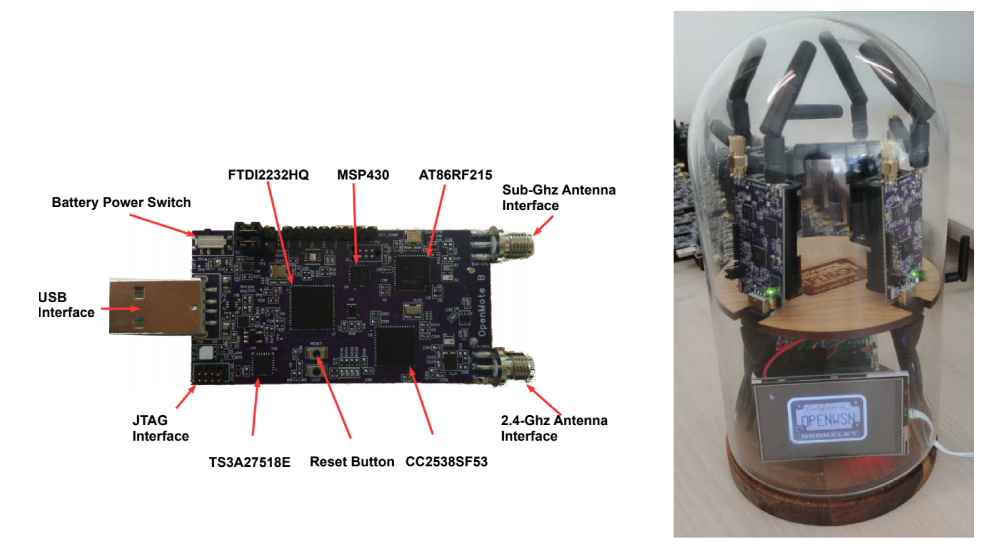
\includegraphics[width=0.90\columnwidth]{mote_ot}
	\caption{
	    The OpenMote~B board \textit{(left)} and
	    the testbox containing four OpenMote~B boards \textit{(right)}.
	}
    \label{fig:mote_ot}
\end{figure}

% 42-mote deployment

The test-bed is composed of 42 motes deployed across the floor of the EVA lab in Inria Paris as shown in Fig.~\ref{fig:building_motes}.
Boxes are distributed to cover the floor, except in room A102 where a cluster of 18 motes are placed in the same room.
This distribution is distinct from the distribution used in~\cite{brachmann19ieee} in that the nodes are distributed much less uniformly across the floor. 
In this distribution, we aim to introduce non-uniformity akin to that of a real world setting.
The reason is that in an industrial plant, such as in~\cite{civerchia17industrial}, sensors are clustered around the locations of machines or production lines where sensor readings are needed for their predictive maintenance.
For example, the authors of~\cite{civerchia17industrial} deploy clusters of sensors around the heavy ashes water pump, seawater pumps, and evaporators. 
The size of clusters varied from 3 wireless sensors per cluster up to 19 wireless sensors per cluster (in the case of the evaporator equipment consisting of multiple pumps). 

\begin{figure}
	\centering
	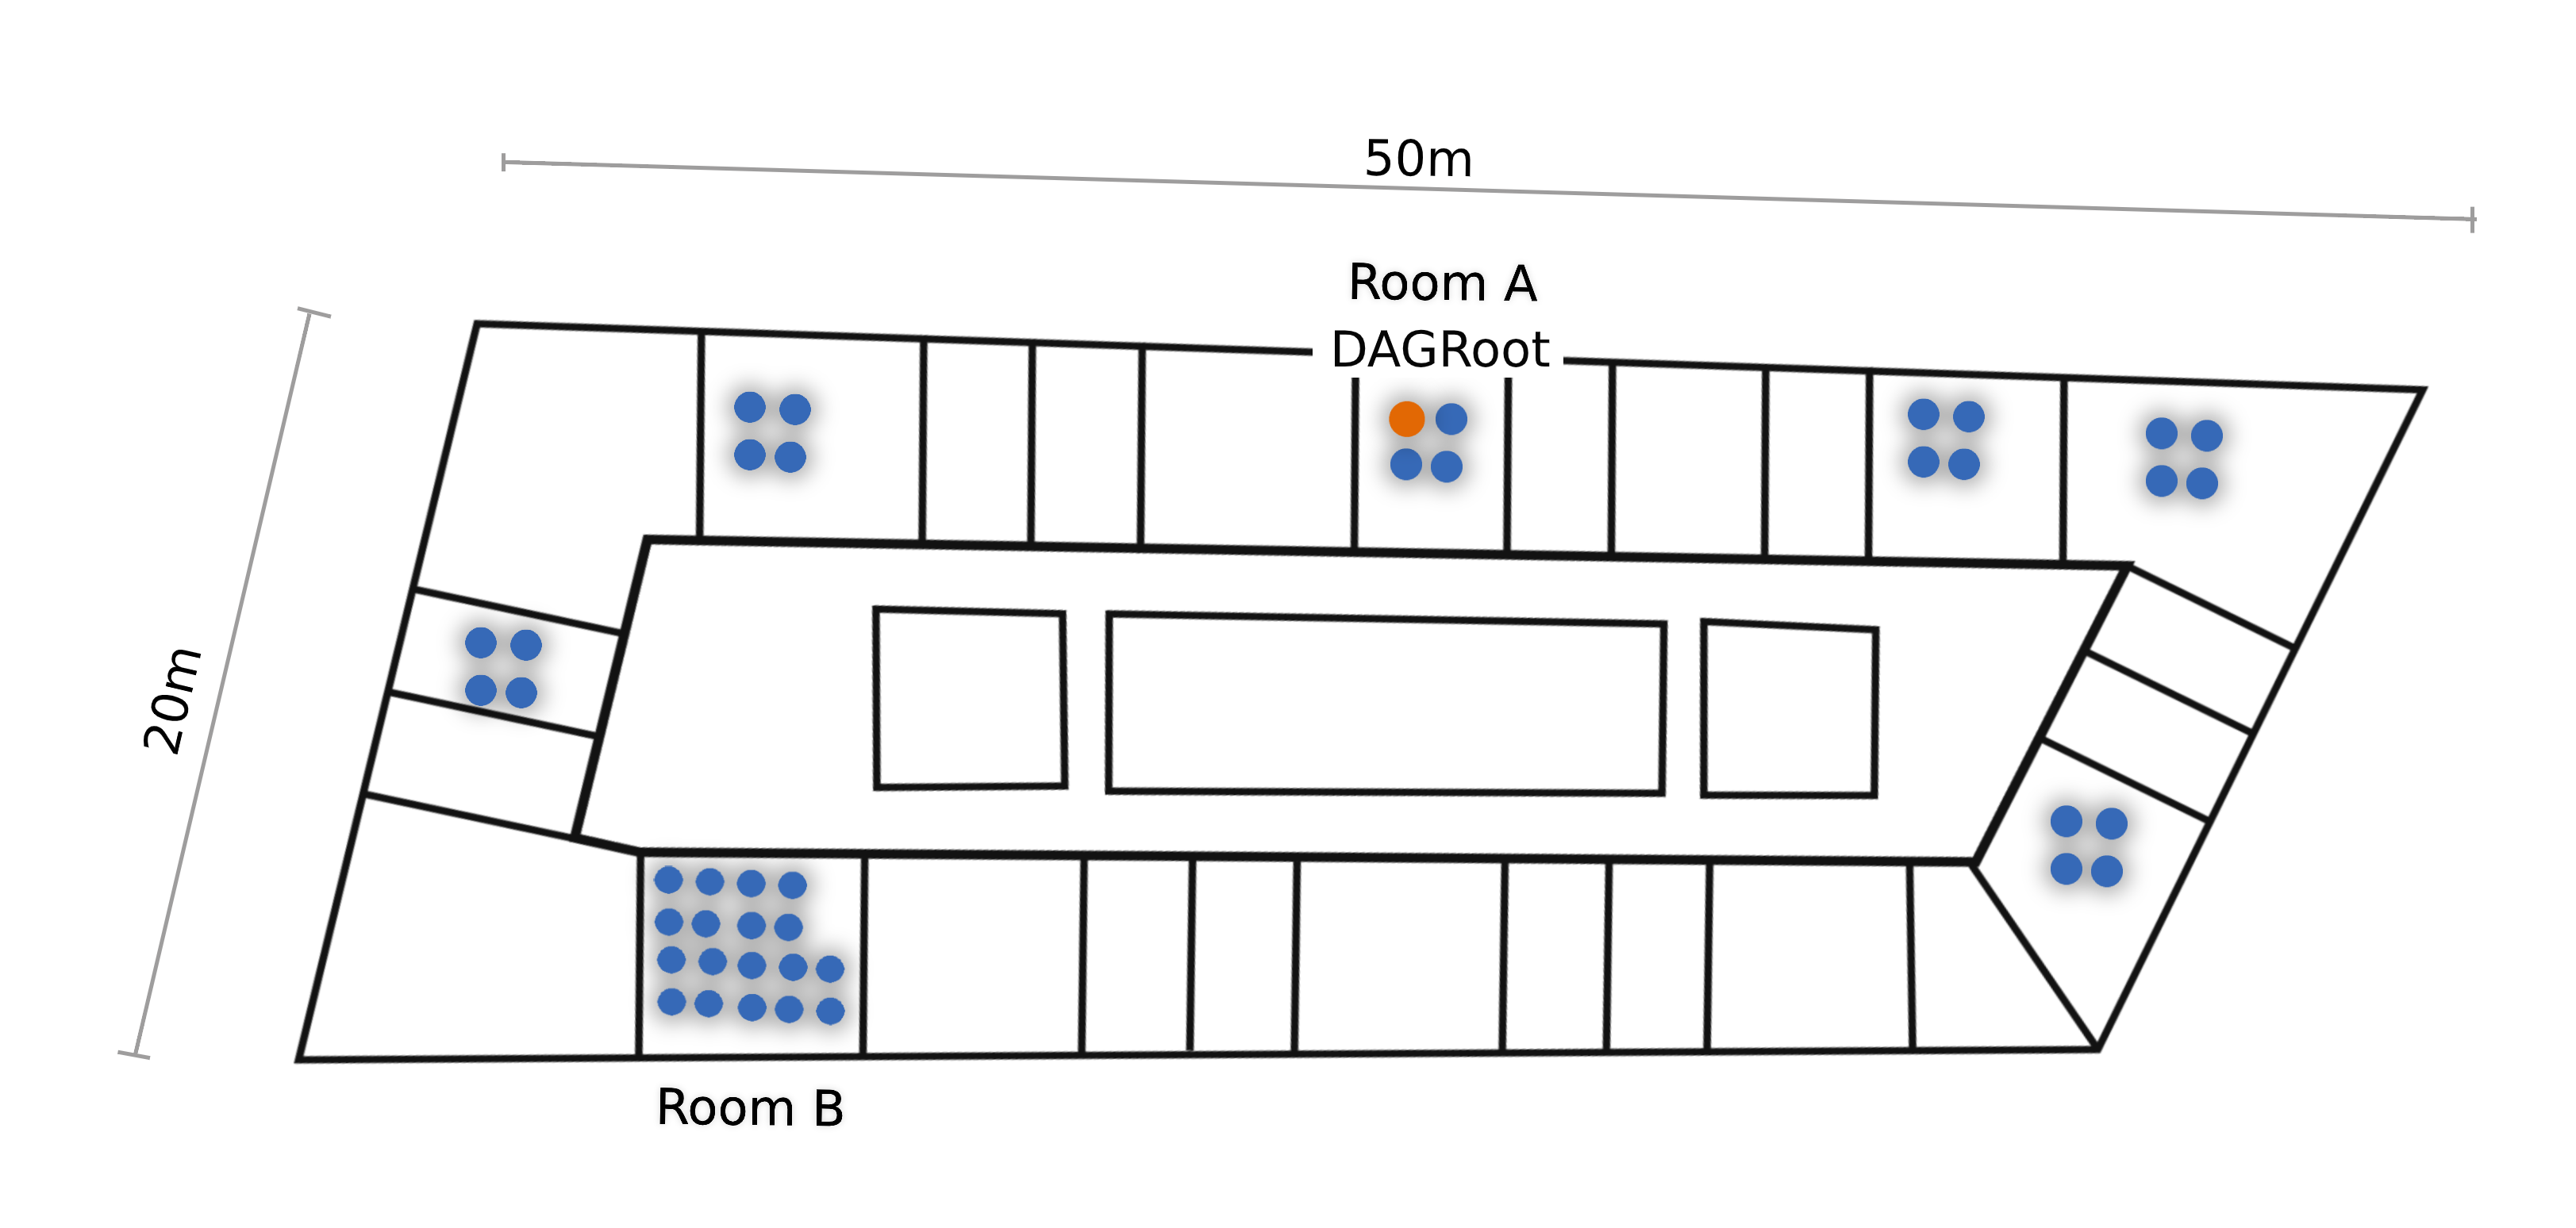
\includegraphics[width=0.85\columnwidth]{building_motes}
	\caption{Floor-plan of the deployment.}
    \label{fig:building_motes}
\end{figure}

%==============================================================================
\section{A PHY-layer Agile Extension of OpenWSN}
\label{sec:openwsn}

% intro to 6TiSCH

In efforts to enable industrial-grade low power wireless networking, the IETF has standardized the set of protocol composing what is now known as the IPv6 over the TSCH mode of IEEE802.15.4e, otherwise known as 6TiSCH~\cite{vilajosana19ietf}.
The 6tiSCH protocol stack is based on IEEE802.15.4 as its PHY and TSCH mode of IEEE802.15.4e as its MAC layer.
Multi-hop capability is supported at the routing layer via the IPv6 routing protocol for Lower-Power and Lossy Networks (RPL). 
Furthermore, 6LoWPAN is an adaptation layer for enabling the interfacing between the routing layer and the specific operations of the MAC layer such as neighbor discovery, registration, ranking, and maintenance operations that impact how routes are calculated. 

% intro to OpenWSN

The 6TiSCH protocol stack has been ported to two main reference architectures: OpenWSN and Contiki-NG. 
Since this work seeks to benefit from the multi-PHY capability of OpenMote~B as explained in section \ref{sec:opentested}, OpenWSN has been selected as the reference architecture for this experiment since it has already been maintained for several boards, including OpenMote~B. 
OpenWSN is an RTOS that allows protocol layers and applications to run side by side on top of a real-time task scheduler implemented based on the interrupt service routine of the microprocessor.
Before the start of this research, OpenWSN was maintained for IEEE802.15.4 O-QPSK 2.4 GHz radio. 
While a driver was available for the At86rf215 radio to pursue the indoor and outdoor range testing in~\cite{munoz18evaluationa} and~\cite{munoz18overview}, two challenges were still unmet: 
    1) OpenWSN has operated based on a single radio-driver only (the CC2538 driver for \oqpsk) . Therefore, if the 6TiSCH stack is to run on different modulations, OpenWSN needs to offer multi-driver support.
    2) IEEE802.15.4e time-slot templates were not derived for the range of modulations to be tested in this experiment.  Therefore, if the 6TiSCH stack is to run on different modulations, OpenWSN needs to offer multi-slot-template support.

% goal: multiple PHY layer

To overcome those challenges, an agile PHY layer is designed for OpenWSN such that the selected radio option at the PHY layer and time-slot template at the MAC layer can change while the rest of the 6TiSCH stack remains intact. 
For this paper, three modulations were selected for the experiment: \fsk, \ofdm, and \oqpsk, each representing the extremes of IEEE802.15.4g modulations as longest range, highest bit-rate, and least power consuming, respectively~\cite{munoz19km}
However, instead of simply hard-coding the radio and MAC parameters in the OpenWSN stack to use the new driver and the respective time-slot, a future-proof ``parameterized'' approach is introduced such that researchers or engineers may adapt the PHY layer freely by simply supplying their slot-templates and radio-drivers as parameters to the RTOS. 

% OpenWSN Extension

To this end, OpenWSN was extended with two capabilities:
1) A generic OpenRadio interface: this interface driver is compliant to the function calls used by the IEEE802.15.4e MAC layer. 
In contrast to a classic driver which executes read/write operations to the radio, it contains a map of function pointers to multiple radio drivers. 
Based on the selected radio option by the MAC layer (for example the \oqpsk on CC2538 or OFDM option 1 MCS3 868 MHz on AT86rf215), the OpenRadio driver redirects the function calls from the MAC layer to the matching function call in the CC2538 driver or AT86rf215 driver. 
2) A time-slot template configuration: three time-slot templates were created in compliance with the IEEE802.15.4e TSCH Information Element (IE) fields.
The templates were derived experimentally by measuring  the communication time to execute commands on the radio chips and  for  and the time on air for a complete data transaction with acknowledgement.
AT86rf215-based options required a longer SPI communication time to be taken into account during Tx/Rx data/ack prepare events. 
This lead to an additional increase in radio duty cycle as well as a decrease in the effective bit-rate at layer 2 due to the the SPI bottleneck at both ends of the link.
Fig.~\ref{fig:openradio} demonstrates the logic analyzer trace of a  transmission of 100B data payload with acknowledgement using the configured time slot for each template. 
Red markers highlight the approximate the time cost of SPI communications which is negligible in CC2538 SoC radio compared to the SPI-connected At86rf215. 
A 40 ms slot template duration is used for all options since it is the minimum for \fsk\. 
Even though \oqpsk\and \ofdm could benefit from a smaller slot duration, a single duration is needed for fair comparison of end-to-end performance using each PHY, specially for time-sensitive metrics such as total radio duty cycle or end-to-end latency.  

\begin{figure}
	\centering
	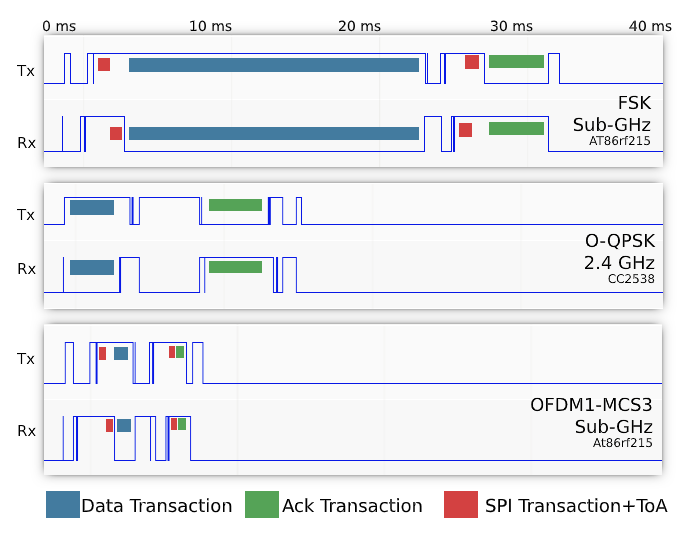
\includegraphics[width=0.49\columnwidth]{openradio}
	\caption{Capture of time-slots during an acknowledged transaction for each PHY layer. Radio duty cycle is extended for FSK and OFDM due to the duration of SPI transactions.}
    \label{fig:openradio}
\end{figure}

% result: footprint

Finally, the footprint of the previous OpenWSN release supporting only \oqpsk\ was 42 kBytes.   
However, the resulting OpenWSN firmware has a memory footprint of 77 kB including the OpenDriver interface, CC2538 radio driver, AT86rf215 radio driver, and the array of supported slot-templates.
This is a low footprint compare to most systems for IIoT such as CC2538 SoC with 512KB flash. 

%==============================================================================
\section{Methodology}
\label{sec:methodology}

% repeating 3 times

OpenWSN is boot-loaded on the OpenTestbed three times where each time the MAC layer selects one of the three radio options in the OpenRadio driver and the respective slot-template. 
The slot frame length is expected to be a prime number to disallow overlapping channel hopping patterns as explained in~\cite{rfc7554}.
Therefore the slot frame length is configured for 41 slots which is slightly less than the number of nodes in the network of 42 to push the system to its scheduling limits. 
Relevant configurations of the protocol stack are presented in table~\ref{tab:stack_config}.
Furthermore, boot-loading is executed on all motes at the same time.
This is expected to maximize the the number of motes trying to join the network and find the best parent at the same time, therefore pushing the network to its limit.
Therefore, this forms a basis for confidence in the performance results as worst-case 

\begin{table}
    \centering
    \begin{tabular}{|l|l|}
        \hline
        Parameter                           & Value  \\ \hline
        Application traffic rate            & 60~s   \\
        RPL DIO period                      & 10~s   \\
        RPL DAO period                      & 60~s   \\
        Max neighbors                       & 45     \\
        Standard packet queue size          & 15     \\
        TSCH Slot-frame length              & 41     \\
        Slot duration                       & 40~ms  \\
        EB probability                      & 0.1    \\
        Radio channels                      & 16     \\
        New neighbor RSSI threshold         & -80~dB \\
        Max re-transmissions                & 15     \\ \hline
    \end{tabular}
    \caption{Protocol stack configuration}
    \label{tab:stack_config}
\end{table}

% duration of one experiment

After boot-loading, the DAG root is set.
The root was chosen in room~A120 which is the closest possible location to the center of the floor Fig.~\ref{fig:building_motes}.
Initial runs show all motes join the network by nearly 15~minutes at 10\% EB probability (equivalent 16~sec EB period).
A node is considered unreachable if a RPL DAO is not received within 15~minutes by the root.
Therefore, it was decided to let the network run for 90~minutes (15x4) to ensure that motes remain reachable for a reasonable duration after the join process. 

% gathering data, publishing raw results, etc.

A UDP application was installed on top of the OpenWSN and was configured to push a packet every 1 minute to the 6TiSCH stack. 
The packets contained the following data fields:

\begin{itemize}
    \item Counter,
    \item Asynchronous Slot Number (ASN) captured at the mote the time of packet composition,
    \item Current DAG rank of the mote,
    \item Neighbor table size,
    \item Total clock ticks the radio is on since the previous packet
    \item Total clock ticks the radio was in transmit state since the previous packet
    \item Total clock ticks passed since the previous packet , and
    \item Maximum and minimum packet buffer occupancy since the previous packet.
\end{itemize}

Once the root receives the packet, it appends to it the current ASN of the root and then writes the array of bytes to the serial port.
The OpenVisualizer (OV) interface~\cite{munoz19opentestbed} parses all packets forwarded from the root tags it with the timestamp and pushes it over MQTT for logging.
The OV keeps track of all RPL DAO packets received by the root and establishes a count of all the motes that has sent a packet within the last 15~minutes and pushes the updates for logging. 

% KPIs

The following KPIs are selected for evaluating the network performance according to~\cite{vucinic20key}:

\begin{itemize}
    \item Network Formation Time: refers to the distribution of the times of arrival of first packet from all motes in the network. 
    \item End-to-End Reliability: refers to the ratio of packets transmitted from all motes to the packets delivered at the root. 
    \item End-to-End latency: refers to the time difference between the triggering of the packet generating event and the time of arrival of the     packet at the root. 
    \item Radio duty cycle:  refers to the ratio of time the radio is powered on, whether in transmit, receive, or idle state.
\end{itemize}

% running the experiments

After execution of each experiment, KPIs are calculated offline from the raw data captures. 
All experiments were executed during lab vacancy to ensure that the results are from the same comparable settings. 
This is particularly important due to the expected interference from Wi-Fi with \oqpsk\ as shown in~\cite{munoz18overview}.

The data is generally reported in three forms:

\begin{itemize}
    \item Time series plot: showing the mean and the inter-quartile range of the KPI in the network during the experiment run with a sliding-window sampling of 3~minutes window-size and one second resolution. 
    \item Cumulative Distribution Function (CDF): showing the cumulative distribution of all the data samples captured for the network at steady state (from minute 30 to the end), at a 100-bin resolution. This allows a fair comparison among the configurations considering all the reported samples.
    \item Probability Distribution Function (PDF): showing the probability distribution of all the data samples at steady state at a 100-bin resolution. This allows a more detailed assessment of the distribution of each data-set. 
\end{itemize}

%==============================================================================
\section{Experimental Results}
\label{sec:results}

This section demonstrates the results of the experiment campaigns.
Each PHY layer offers link budget as detailed in table \ref{tab:linkbudget}. 
Each subsection demonstrates how PHY layer properties affect the end-to-end performance results. 

\begin{table}
    \centering
    \begin{tabular}{|l|l|l|l|}
        \hline
                & Tx power (max) & Rx sensitivity & Link budget \\ \hline
        \fsk\   & +14~dBm        & -114~dBm       & 128~dB      \\ \hline
        \ofdm\  & +10~dBm        & -104~dBm       & 114~dB      \\ \hline
        \oqpsk\ & +7~dBm         & -97~dBm        & 104~dB      \\ \hline
    \end{tabular}
    \caption{Link characteristics for each PHY layer.}
    \label{tab:linkbudget}
\end{table}

%------------------------------------------------------------------------------
\subsection{Network Formation}
\label{sec:network_formation}

% why is it important, define

Network formation KPI is defined as the time-to-first-packet  from all motes in the network.
It is evaluated as the CDF of the time elapsed since initializing the DAG root until packet reception. 
This parameter is relevant to reflect the expected time for network installation since in some applications such as industrial settings, installation time could come at a cost of labor and/or withholding production operations.

% worst case from a contention point of view

Network is formed as nodes establish secure join handshakes with a synchronized member of the network.
The rate at which the network is formed depends on whether nodes are joining gradually or  simultaneously.
The reason is that join requests are established via shared cells, therefore a burst of join requests to a common neighbor leads to delay in the join process based on random back-off exponents. 
To allow a fair comparison among the three modulations, it is decided to maximize the contention in the network in a worst-case scenario by boot-loading all the motes simultaneously as explained in section \ref{sec:methodology}.

% results: why is it affected by link budget? 

It can be observed in Fig.~\ref{fig:time_firstpacket_cdf} that there is an inverse correlation between link-budget and the rate of network formation. 
The first packet is received from  90\% of the motes within 7, 9, and 11~minutes with \fsk\ , \ofdm\ , and \oqpsk\ respectively. 
The network forms faster with higher link budget PHY layer for two reasons. 
First, nodes discover more neighbors and therefore  it takes less time to hear a synchronized node. 
Second, nodes have higher chance of finding a parent closer to the root (i.e. with lower DAG rank), if not the root itself and this decreases the number of hops necessary for an end-to-end packet delivery.
This leads the network to reach a steady state with 1) generally higher neighbor reach and 2) lower hops to the root. 
This is verified in the following subsections.

\begin{figure}
	\centering
	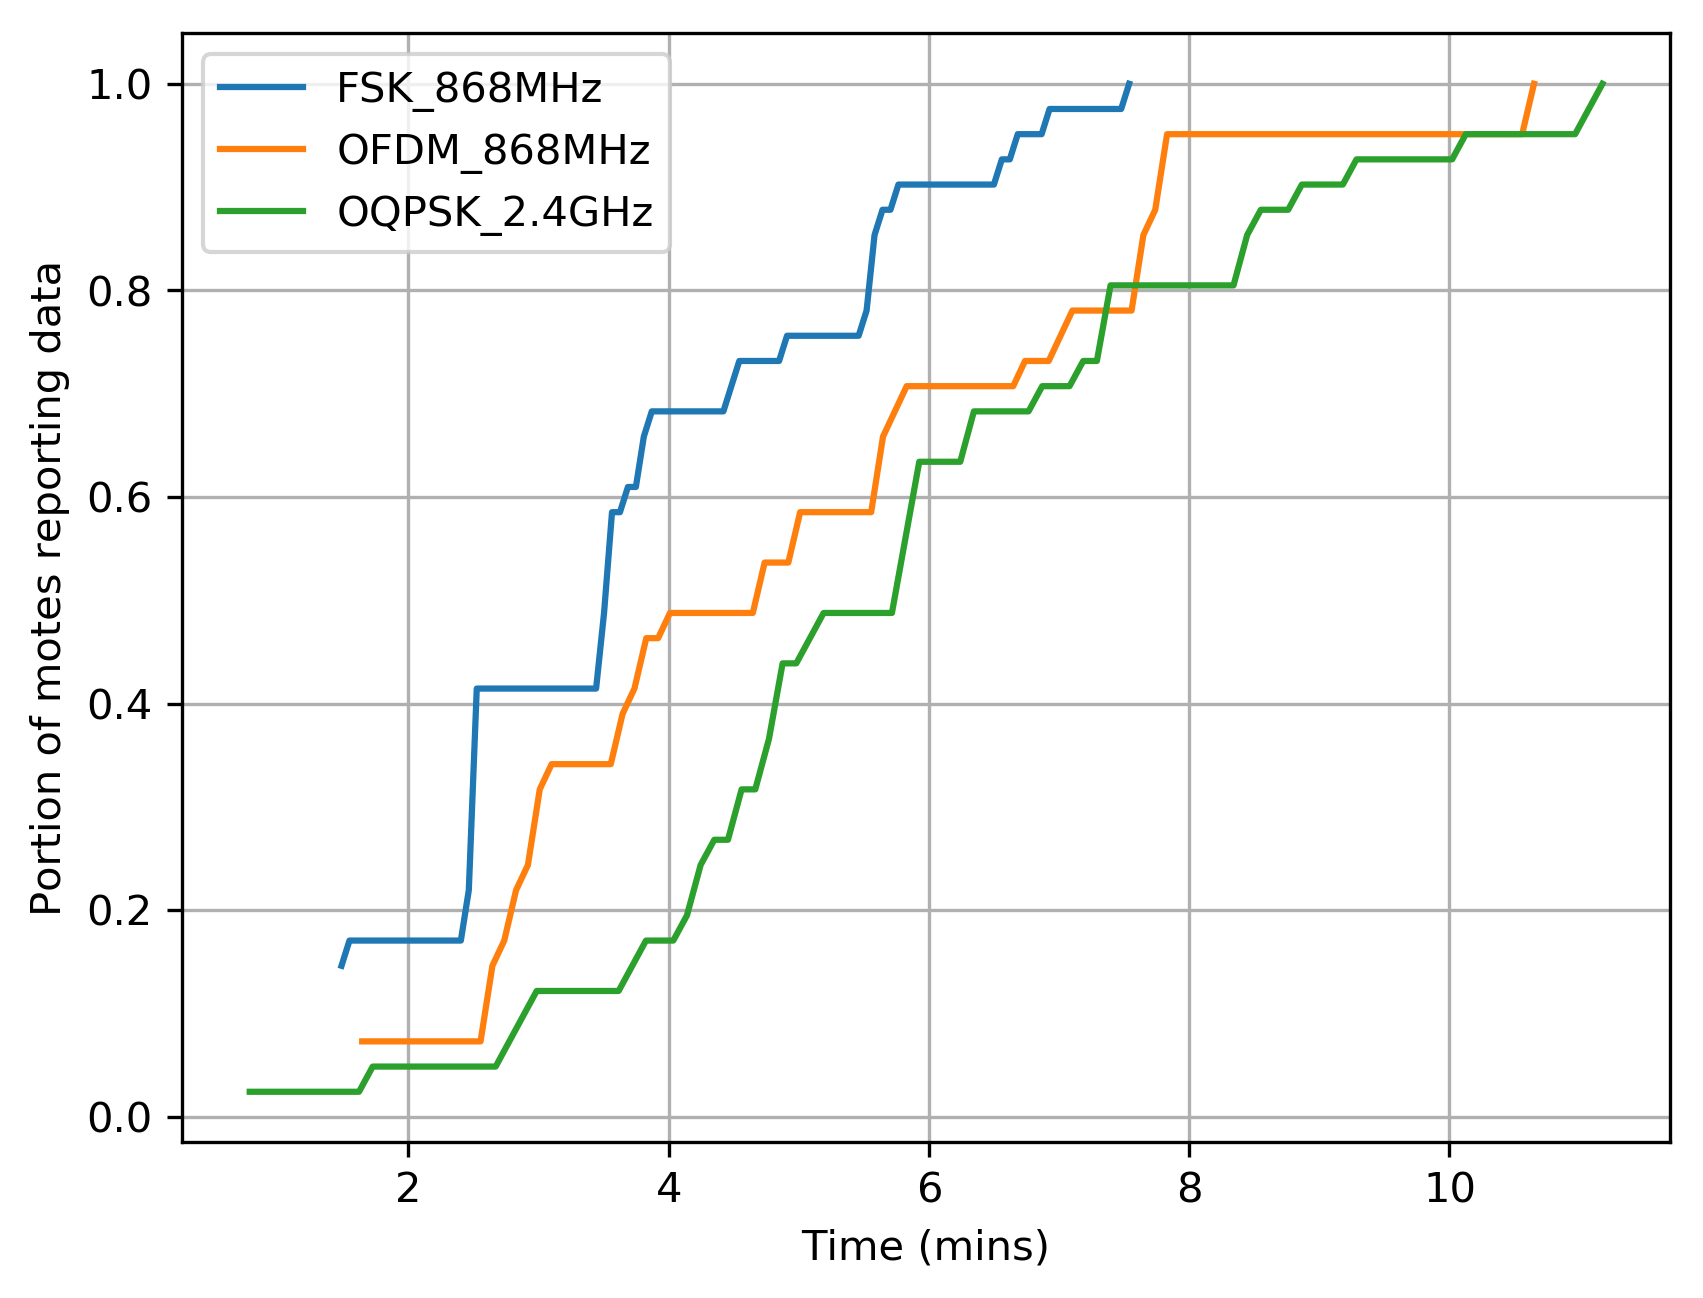
\includegraphics[width=0.45\columnwidth]{time_firstpacket_cdf}
	\caption{Time to First Packet CDF.}
    \label{fig:time_firstpacket_cdf}
\end{figure}

% settling time, steady-state  

% - - - - - - - - - - - - - -
\subsubsection{Neighbor Reach}
\label{sec:neighbor_reach}

% what does it mean

This metric is defined as the total number of neighbors registered in the neighbor table at the time the sample is collected.
It is affected by PHY layer link budget because neighbors registered if a packet has been received with RSSI~$> -80$~dB. 
Therefore, the higher the link budget, the higher the chance that more neighbors are discovered. 

% how is it affected by link budget

The impact of the PHY layer on neighbor reach can be observed in Fig.~\ref{fig:neighbors_all}: the mean and inter-quartile range of discovered neighbors (Fig.~\ref{fig:neighbors_time}) accelerate faster in an inverse correlation with link budget.
By minute 30, an average mote has discovered slightly more than half of the network with \fsk\ , and still in increase until one hour later.
The range of \ofdm\ overlaps with \fsk\ even though it is 16 times faster in bit-rate; also it is better than \oqpsk\ by nearly 35\%  even though it is 3 times faster in bit-rate. 
This is verified in Fig.~\ref{fig:neighbors_cdf} as the CDF of all the data samples in steady state shows the inverse correlation between the number of neighbors and the link budget. 
The PDF in Fig.~\ref{fig:neighbors_pdf}  shows high neighbor reach for \oqpsk only in a dense setting: a cluster around 25 neighbors in room A102 and a cluster around 14 neighbors in nearby rooms

% conclusion pros and cons

Therefore, on one hand, a high link budget PHY-layer leads to faster network formation yet with a possible risk of neighbor table overflow in case of dense deployments.
This risk is significant because there is no standardized mechanism to accept any new neighbor (even if it is a ``better'' one) in case neighbor table is saturated -- as outlines in the IETF RFC~\cite{rfc8505}. 
On the other hand, a low link budget PHY-layer may lead to slower network formation, yet it is useful in dense deployments where motes need to discover only nearby neighbors. 

\begin{figure}
	\centering
	\begin{subfigure}{0.49\columnwidth}
    	\centering
    	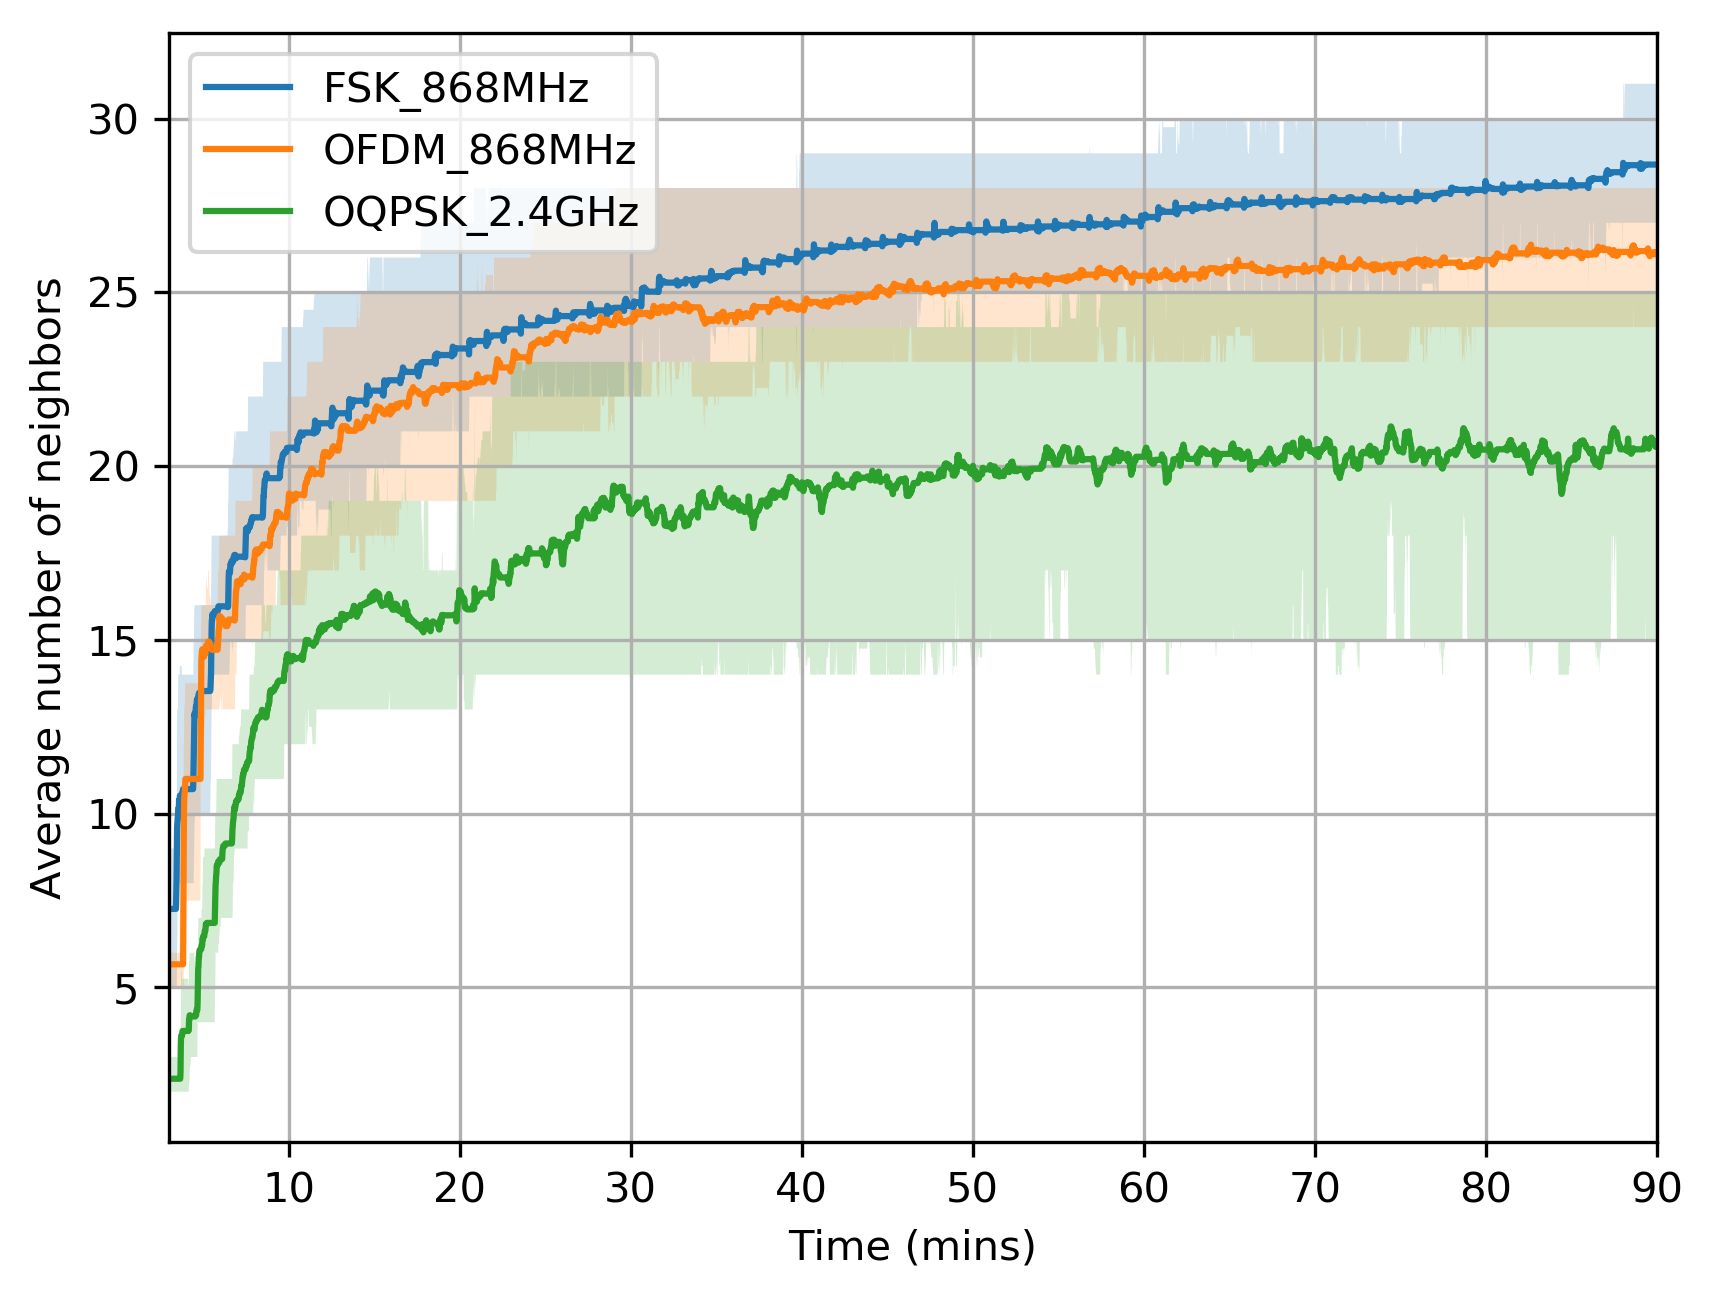
\includegraphics[width=1.00\columnwidth]{neighbors_time}
        \subcaption{Mean and inter-quartile range of measurements in the time domain }
        \label{fig:neighbors_time}
	\end{subfigure}
	\begin{subfigure}{0.49\columnwidth}
		\centering
    	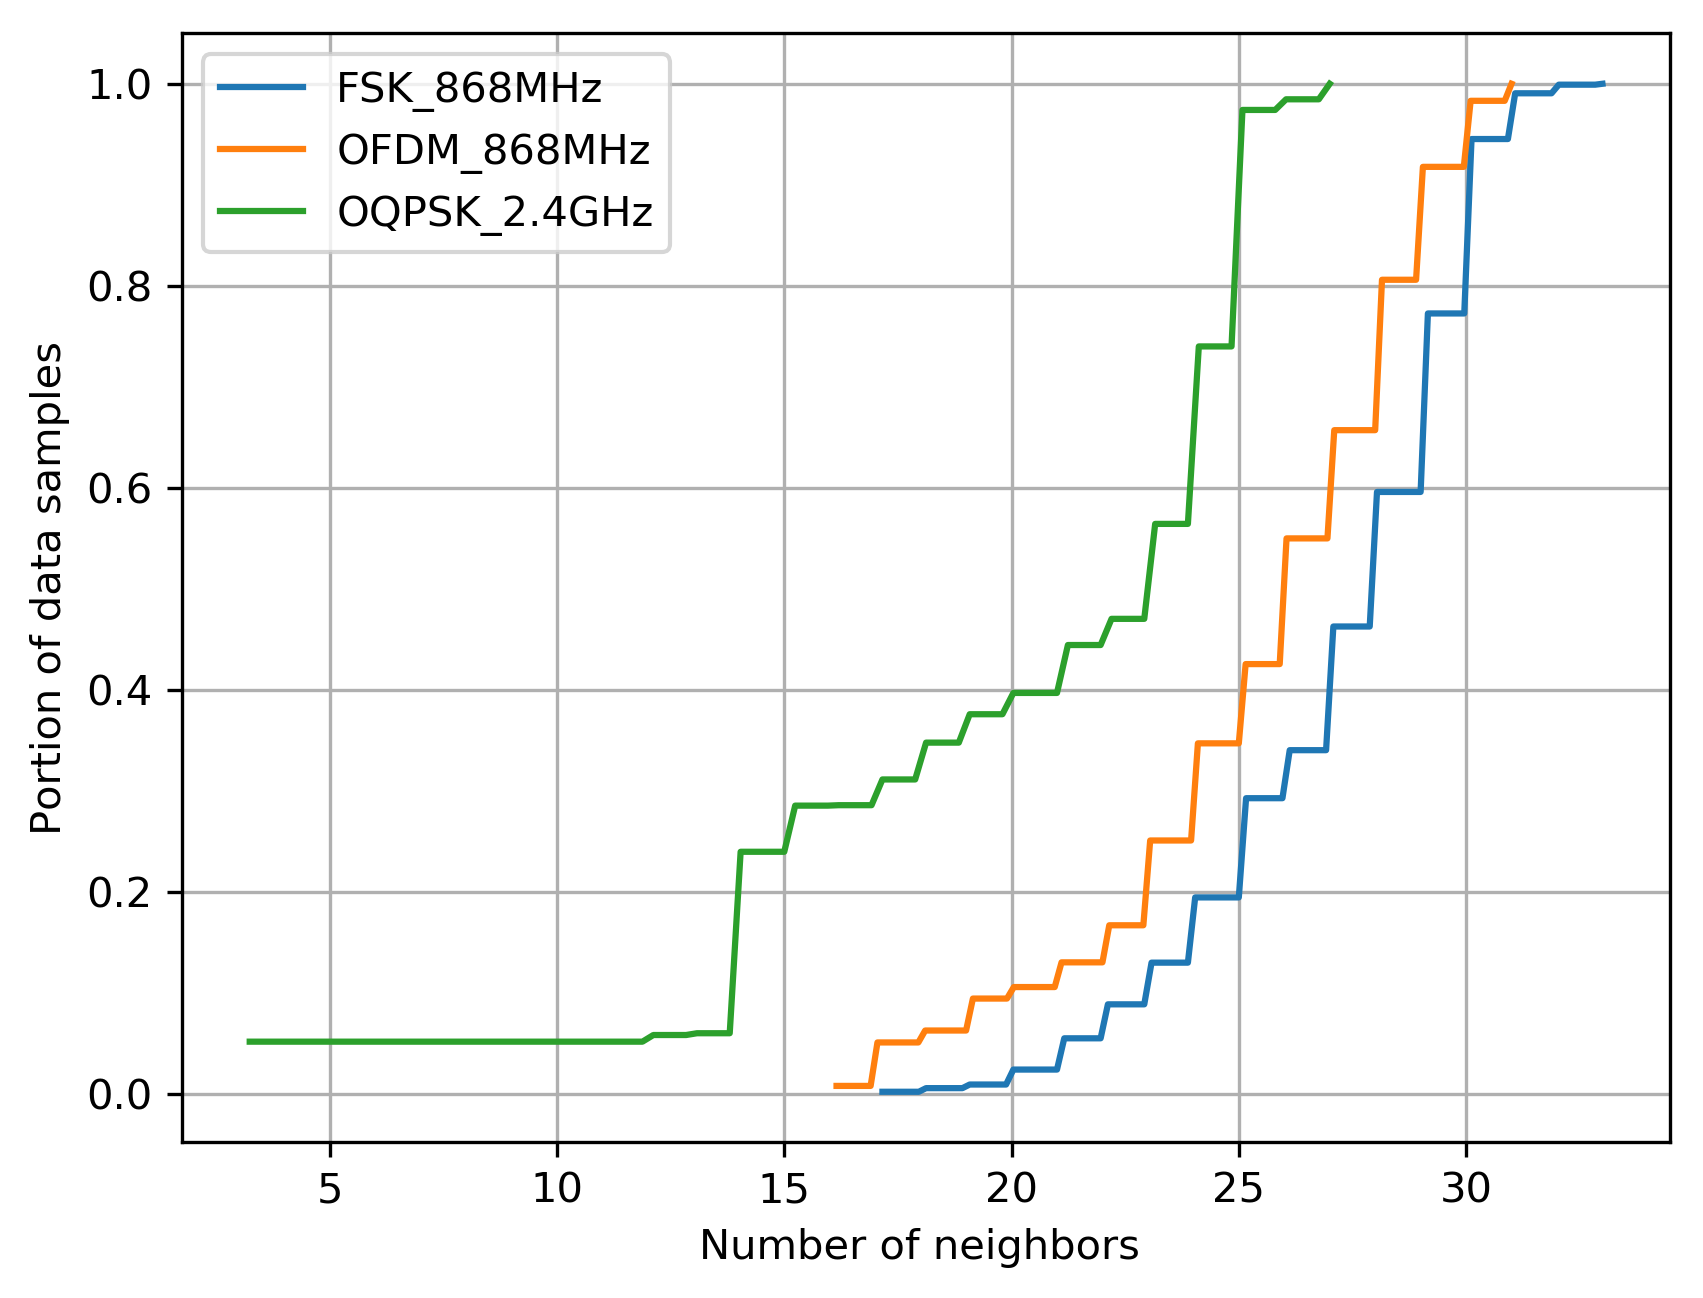
\includegraphics[width=1.00\columnwidth]{neighbors_cdf}
    	\subcaption{CDF of  the measurements for the network at steady state }
        \label{fig:neighbors_cdf}
	\end{subfigure}
	\begin{subfigure}{0.49\columnwidth}
		\centering
    	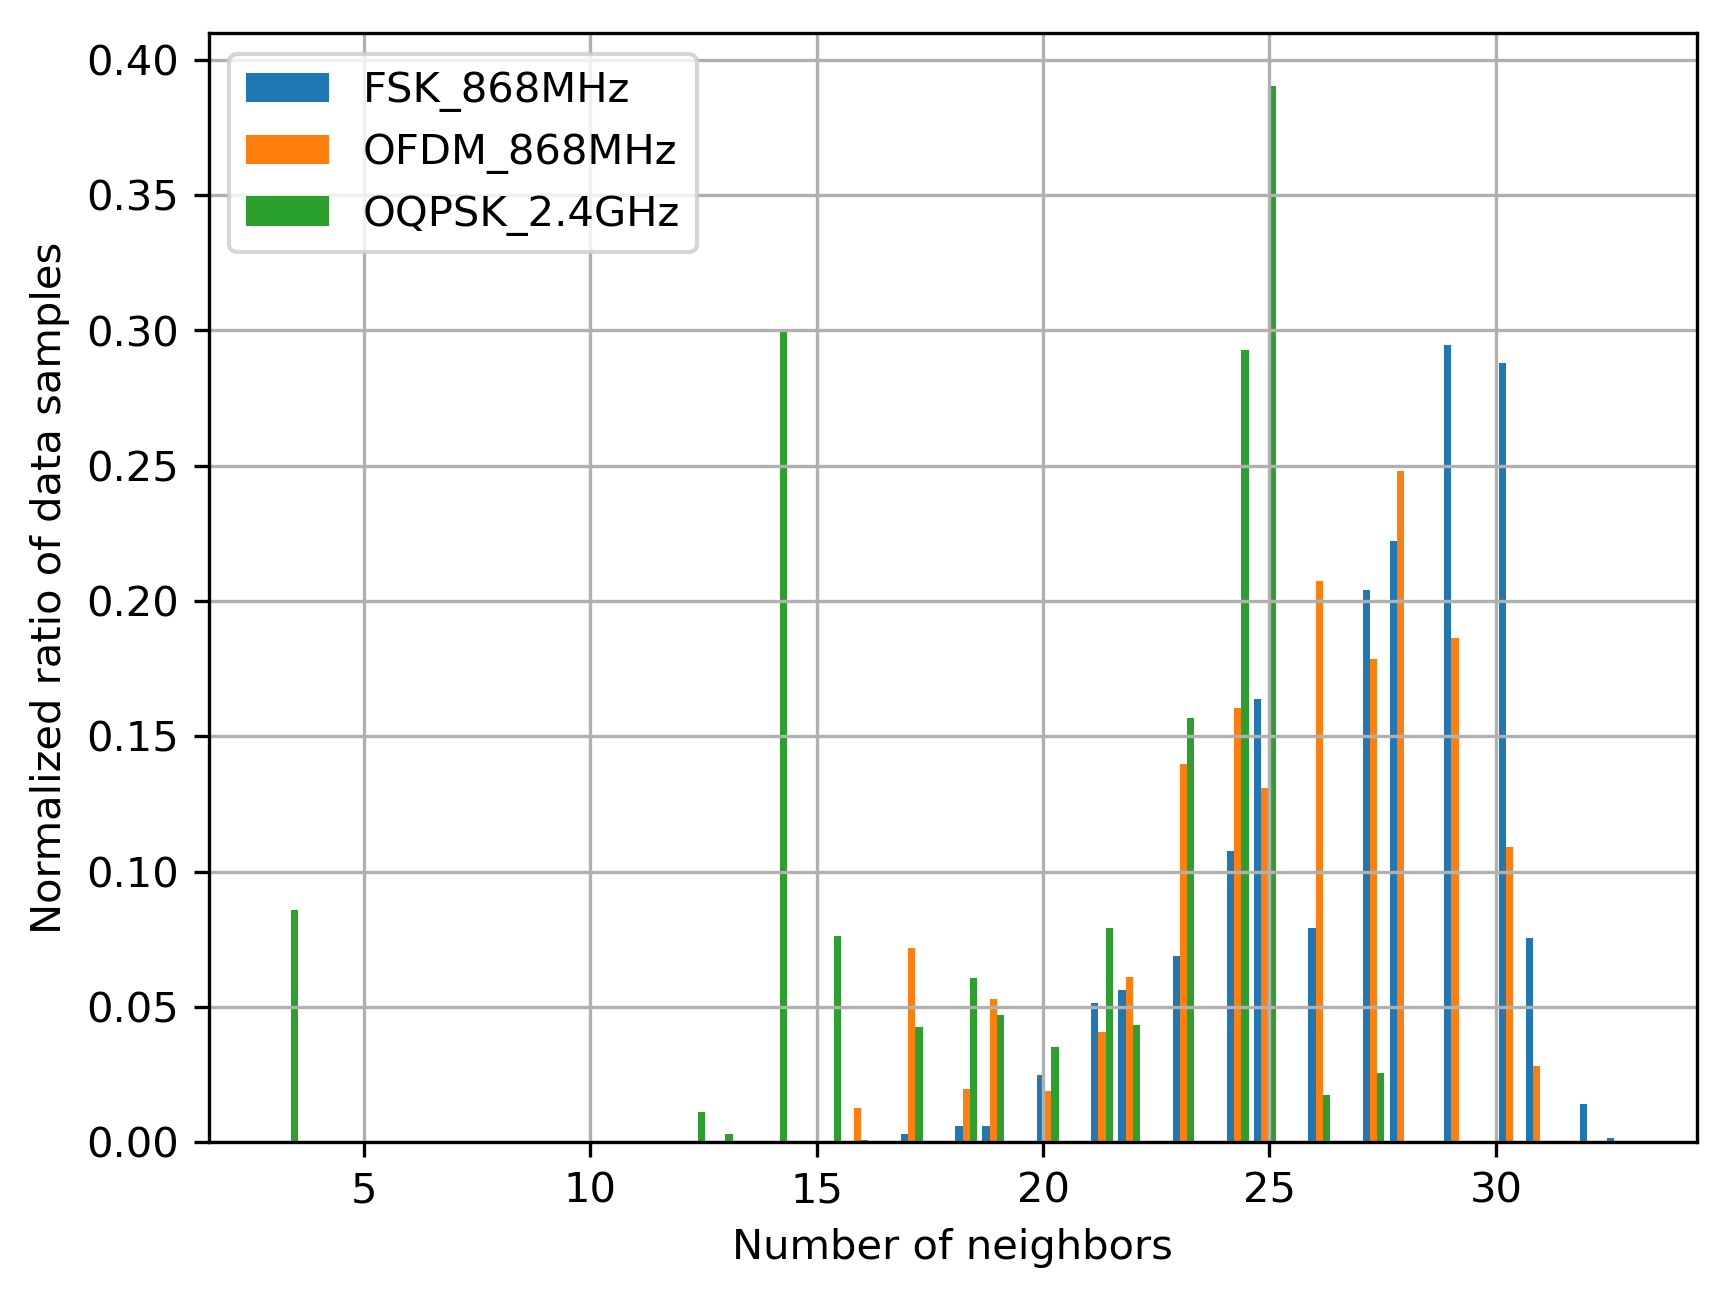
\includegraphics[width=1.00\columnwidth]{neighbors_pdf}
    	\subcaption{PDF of  the measurements for the network at steady state }
    	\label{fig:neighbors_pdf}
	\end{subfigure}
	\caption{
	    Reported number of neighbors in the network.
	    The higher the link budget, the more neighbors are discovered by the 6LoWPAN adaptation layer.
	} 
	\label{fig:neighbors_all}
\end{figure}

% - - - - - - - - - - - - - -
\subsubsection{DAG root reach}
\label{sec:dagroot}

% What does DAG rank mean and Why it means less hops? 

This metric is calculated at the mote at the RPL layer as a function of the expected transmission count (eTx) for the links leading to the root, and it is summed at each hop.
In the current implementation, the rank is calculated as $rank = ((3\times numTx/numAck)-2)-minHopIncrease$, where $minHopeIncease = 256$. 
An important feature of the DAG rank is that it monotonically decrease as  the node approaches the DAG root, as mandated by the RPL standard~\cite{rfc6550}.
Therefore, lower DAG ranks imply overall better path quality either in the number of hops or eTx or both. 

% why does it improves by link budget

A higher link budget at the PHY layer leads to an improved DAG rank and shorter paths to the root as it reduces the need for re-transmissions and for relaying; which leads to faster network formation
It can be observed in Fig.~\ref{fig:dagrank_time} that \fsk maintains, generally, the lowest DAG ranks during network formation as well as late steady state. 
Link budget seems to be inversely correlated with the distribution of the DAG rank in the network as observed in Fig.~\ref{fig:dagrank_cdf}: \fsk\ demonstrates the highest DAGrank at steady state for 90\% of the motes as shown in, followed by \ofdm\ and \oqpsk\ respectively.
This observation is stressed in Fig.~\ref{fig:dagrank_pdf} which shows that the center of the distribution of the \fsk is at the absolute lowest rank possible while the distributions of \ofdm\ shifts to higher ranks followed by \oqpsk. 

% conclusion pros and cons 

Therefore, a higher link budget PHY-layer leads to improved DAG ranks and faster network formation, yet it creates a risk of overloading nodes with good DAG ranks (closer to the root) with scheduling requests 
Since these requests are established on shared cells, they may cause contention leading to energy waste and potentially packet loss -- which is exacerbated in dense deployments.

\begin{figure}
	\centering
	\begin{subfigure}{0.49\columnwidth}
    	\centering
    	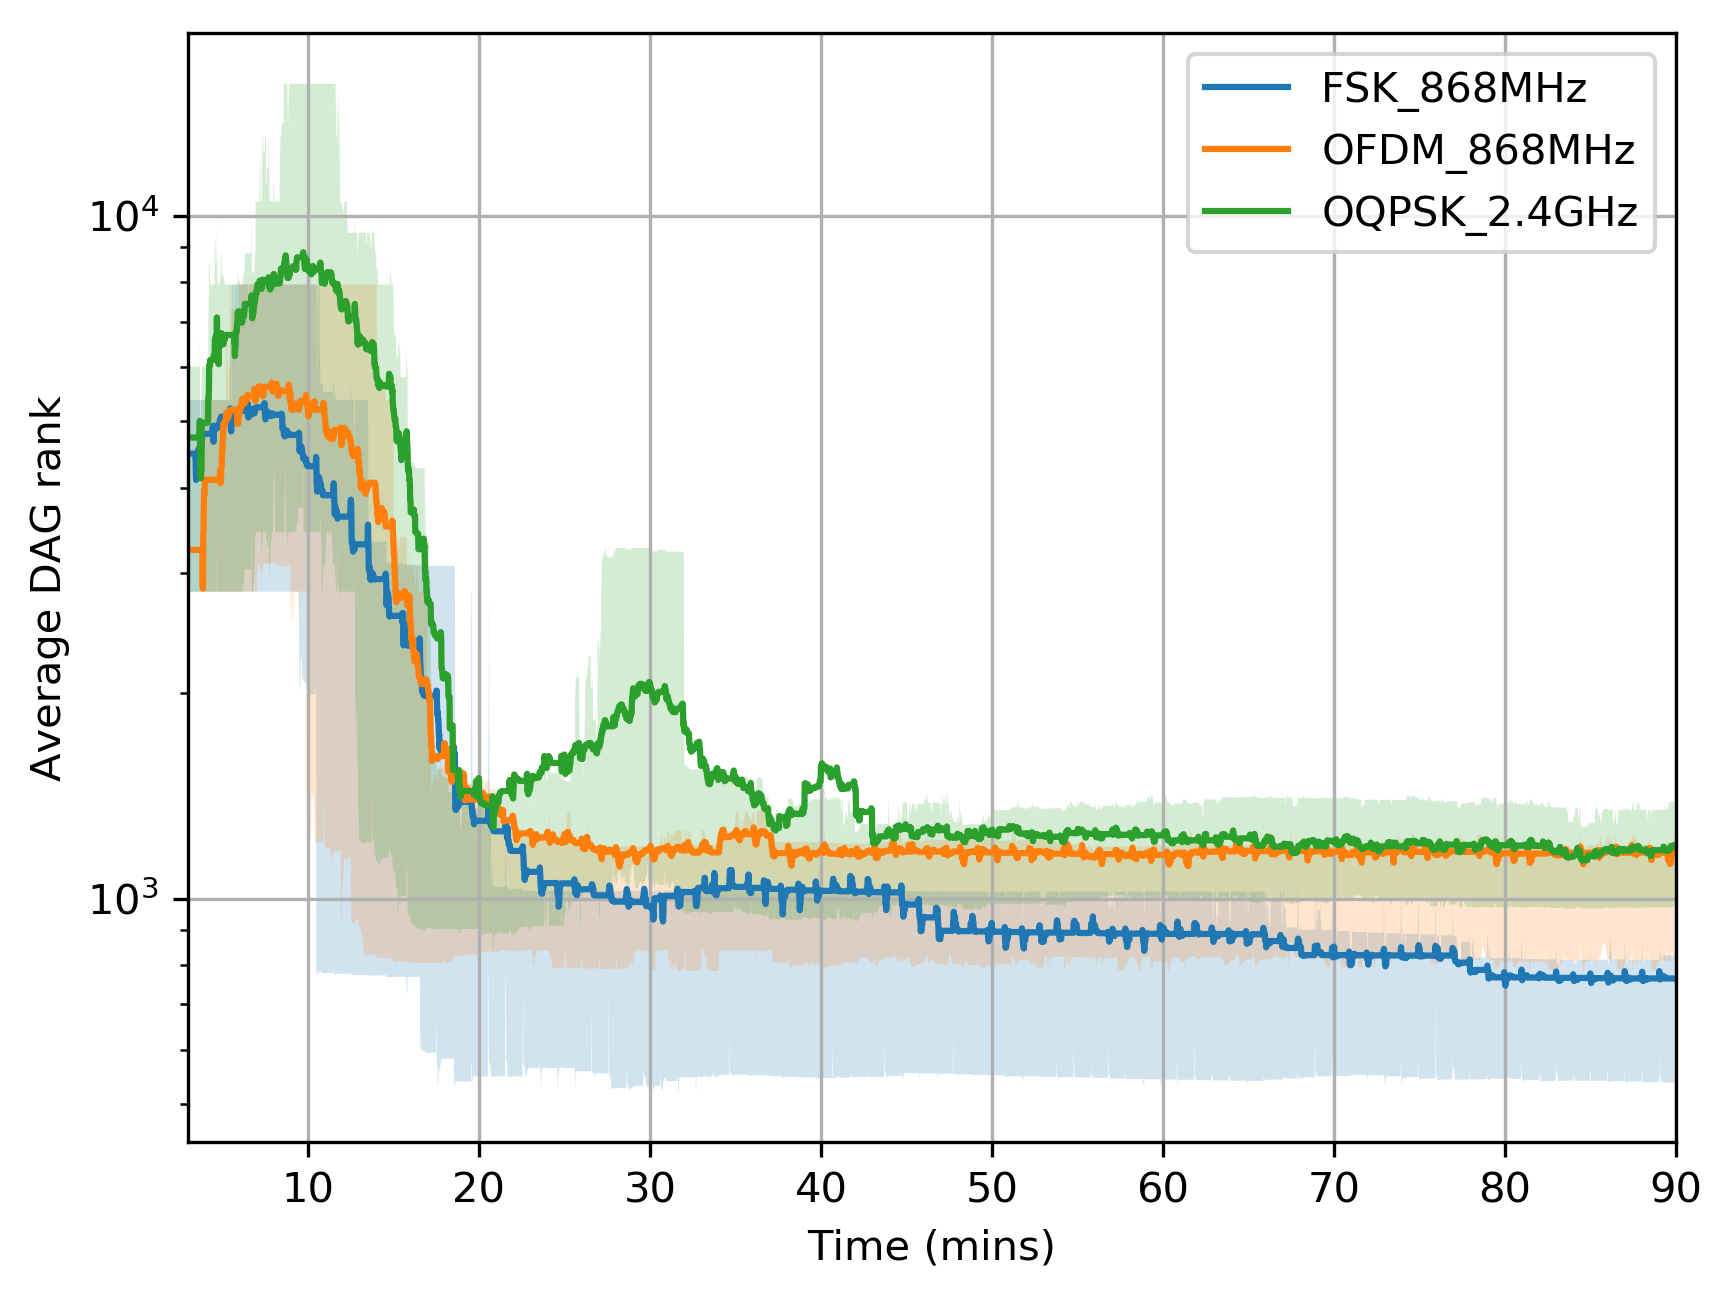
\includegraphics[width=1.00\columnwidth]{dagrank_time}
        \subcaption{Mean and inter-quartile range of measurements in the time domain }
        \label{fig:dagrank_time}
	\end{subfigure}
	\begin{subfigure}{0.49\columnwidth}
		\centering
    	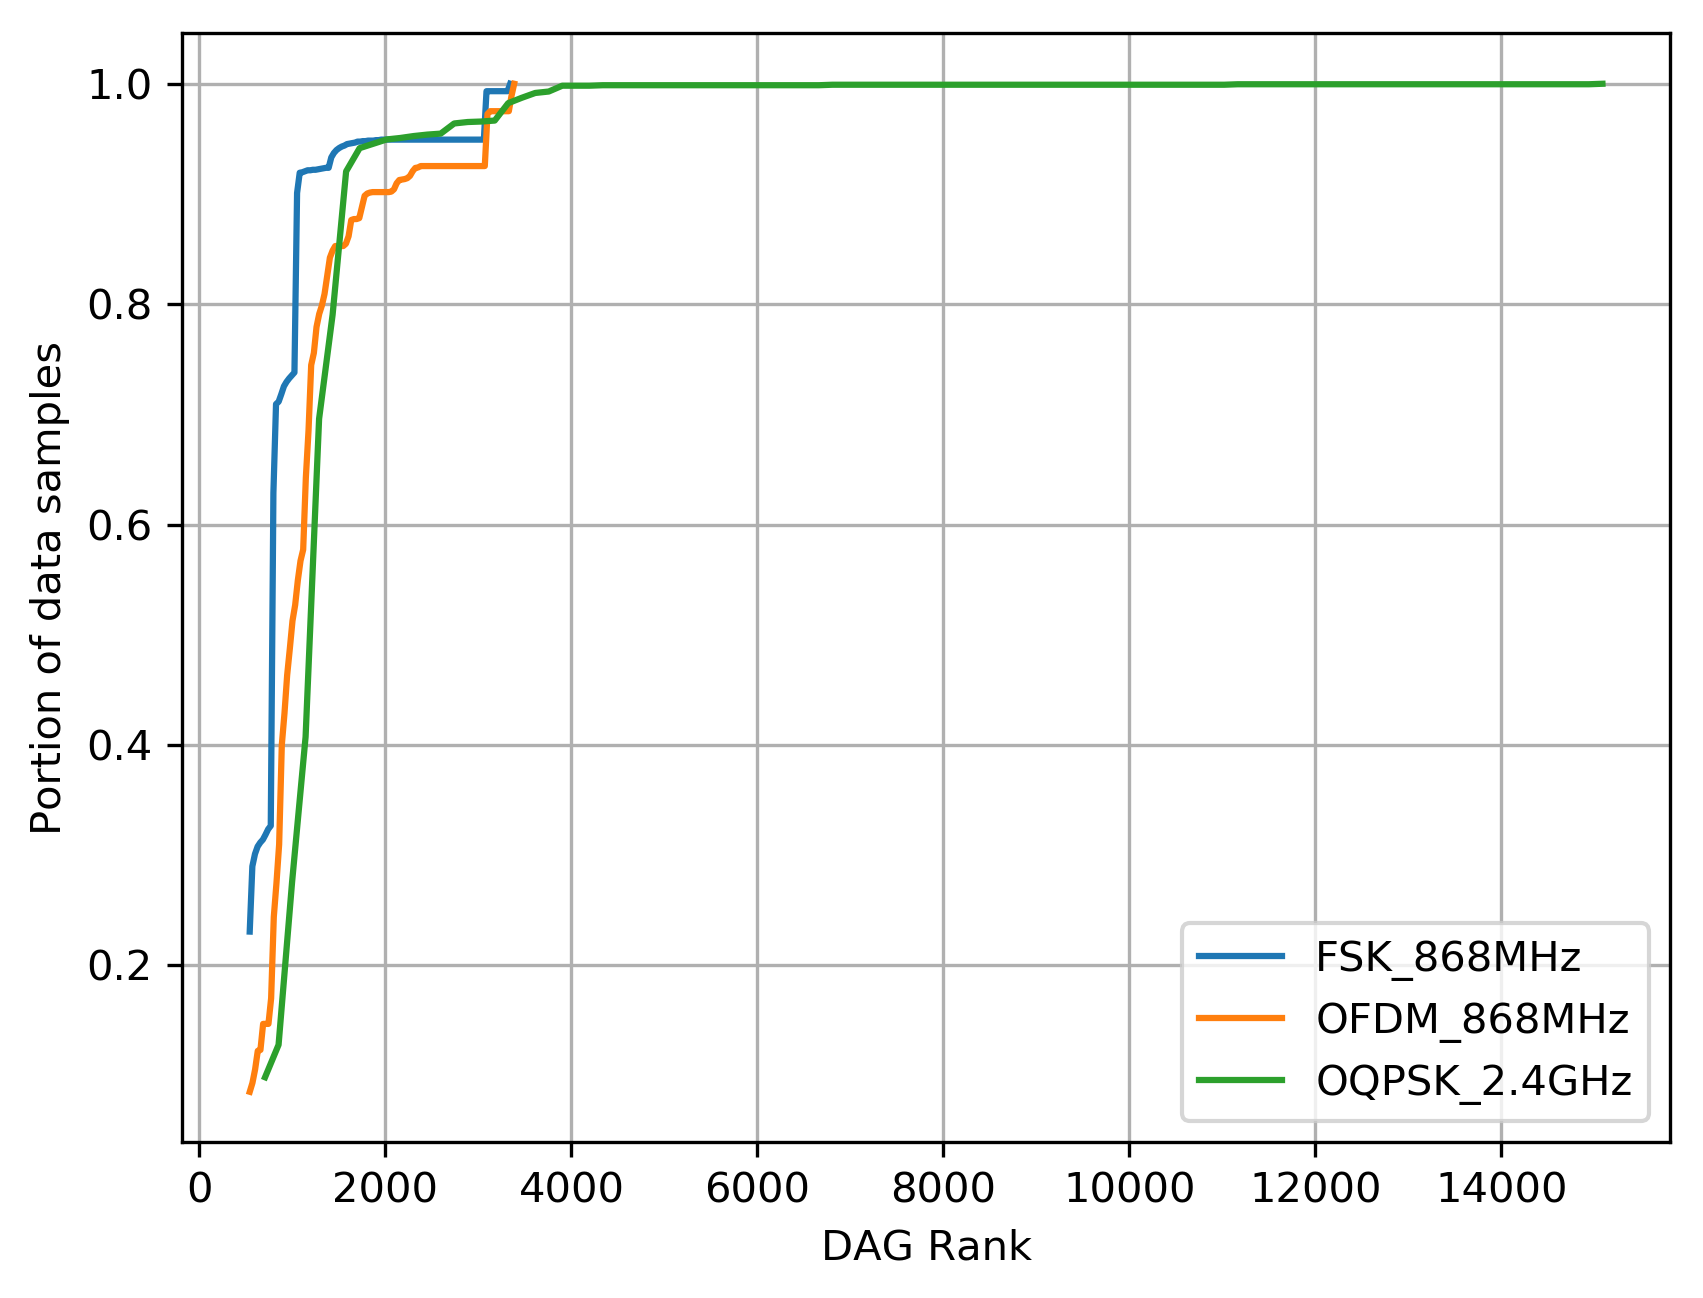
\includegraphics[width=1.00\columnwidth]{dagrank_cdf}
    	\subcaption{CDF of  the measurements for the network at steady state }
        \label{fig:dagrank_cdf}
	\end{subfigure}
	\begin{subfigure}{0.49\columnwidth}
		\centering
    	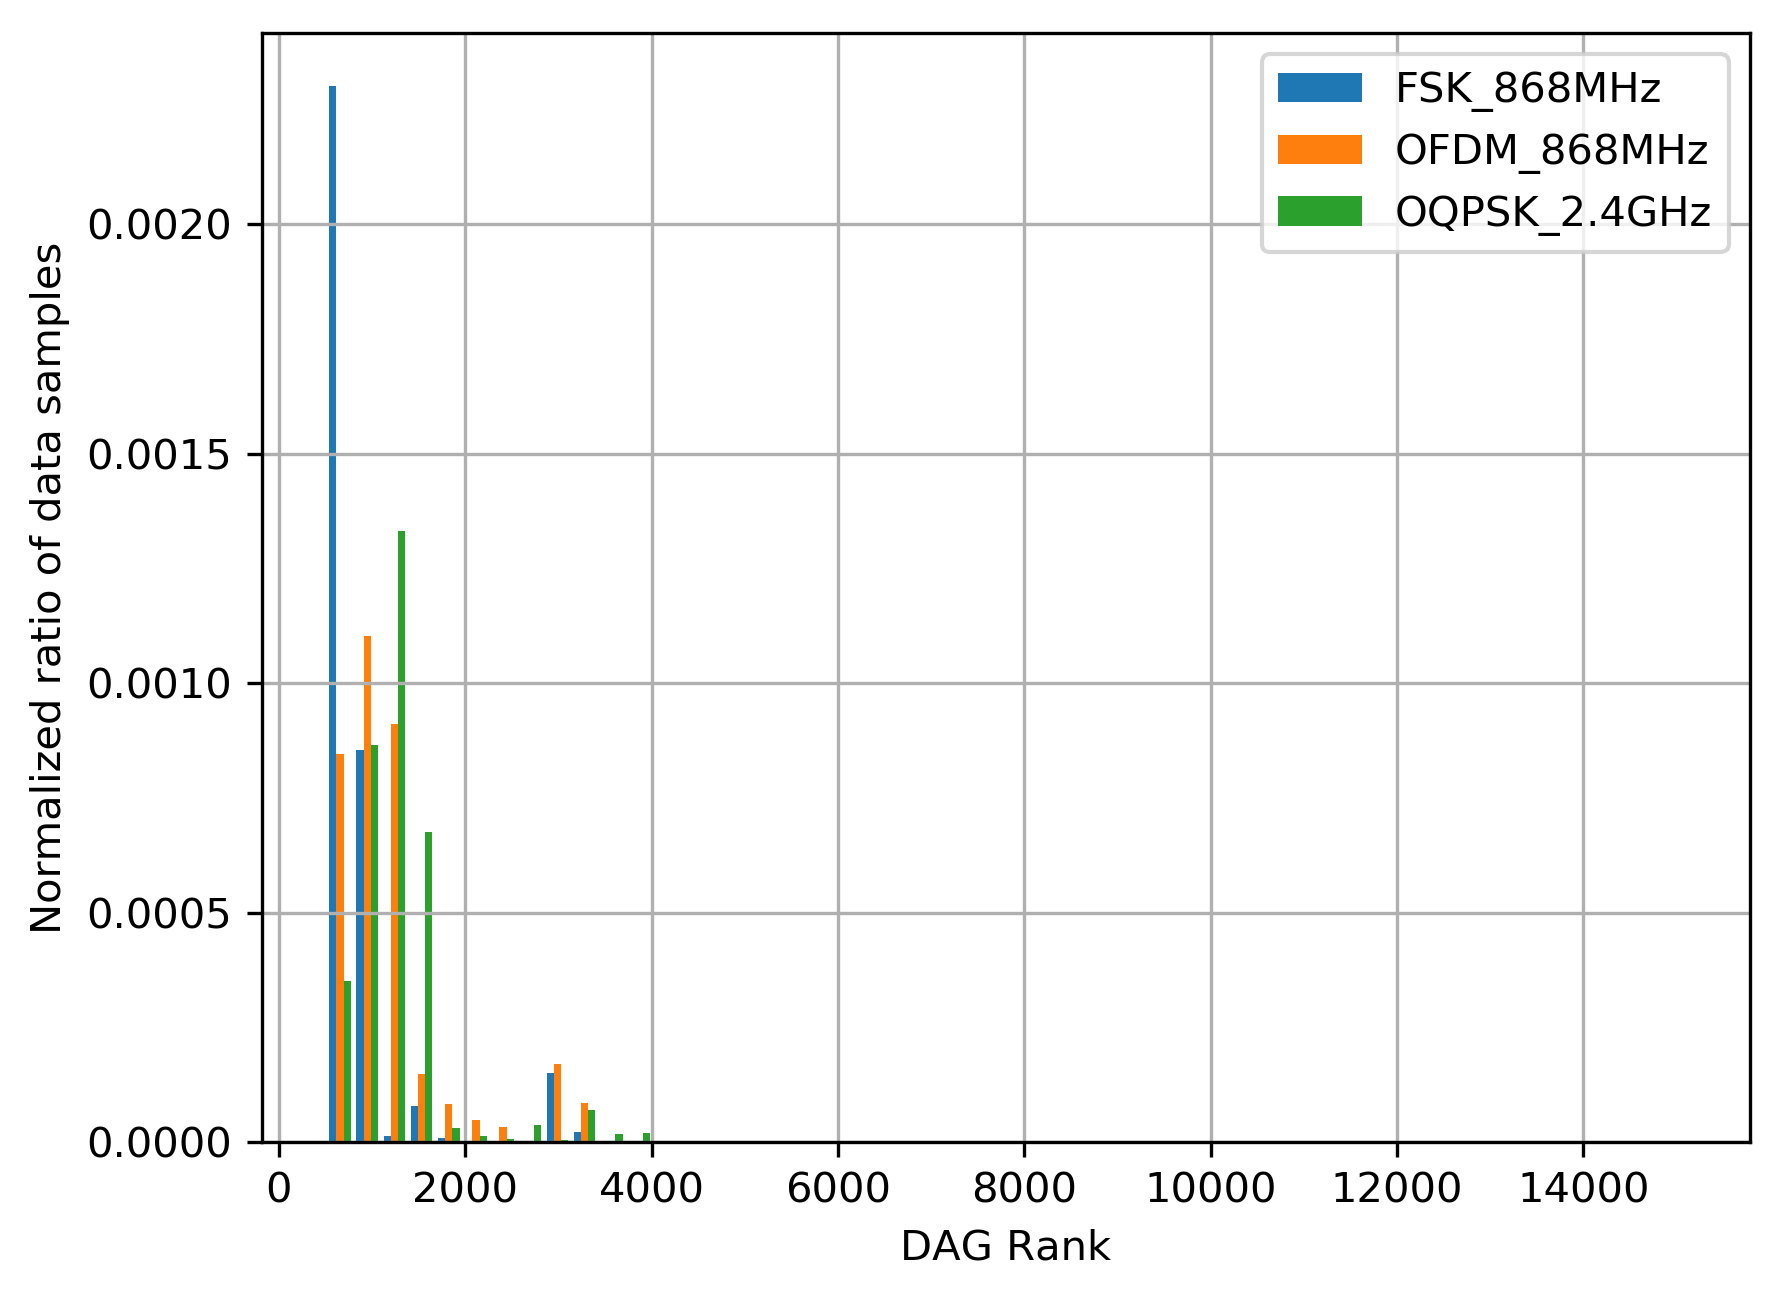
\includegraphics[width=1.00\columnwidth]{dagrank_pdf}
    	\subcaption{PDF of  the measurements for the network at steady state }
    	\label{fig:dagrank_pdf}
	\end{subfigure}
	\caption{
	    Reported DAG Ranks in the network.
	    The higher the link budget at PHY layer, the better the DAG rank and the faster the root can be reached.
	} 
	\label{fig:dagrank_all}
\end{figure}

%------------------------------------------------------------------------------
\subsection{End-to-End Reliability}
\label{sec:reliability}

% what is it and how is it measured

This KPI is measured as the end-to-end PDR of the UDP packets from each mote.
The OV tracks packets received by the root and counts missing packets between the first and last received packets from each mote.
In case a mote is no longer sending packets (or no longer reachable), the PDR would remain as the last updated count.

% another metric needed, but won't be considered? 

Another metric is captured at the root to ensure that unreachable motes are detected: the number of motes that have sent a RPL DAO within the last 15~mins (i.e. ``active motes'').
The reason those two metrics remain separate is that a mote may choose to change parent during its lifetime.
In this case, it may not be able to forward the packets while the negotiation is still in process, which is subject to contention and back-off.
In this case, the packet is not lost necessarily since the mote would keep it in the buffer until a schedule is negotiated with the parent. 
However, this factor is reported for accuracy but will not be addressed in the scope of reliability since it reflects the impact of contention and not necessarily the total loss of packets; alternatively, the focus is on the end-to-end PDR. 

\begin{table}
    \centering
    \begin{tabular}{|l|l|l|l|l|l|l|}
        \hline
                & Average & Median & Min     & Max   & StDev & Active motes \\ \hline
        \fsk\   & 100\%   & 100\%  & 100\%   & 100\% & 0     & 92.8\%       \\ \hline
        \ofdm\  & 99.84\% & 100\%  & 93.75\% & 100\% & 0.9\% & 100\%        \\ \hline
        \oqpsk\ & 98.08\% & 100\%  & 73.3\%  & 100\% & 6\%   & 97.6\%       \\ \hline
    \end{tabular}
    \caption{Steady-state end-to-end PDR values}
    \label{tab:pdr_table}
\end{table}

% Results, there is PDR

Table~\ref{tab:pdr_table} shows PDR values for each configuration for the steady state in the last 15~minutes of the experiment run. 
It shows that link budget is in inverse correlation with end-to-end reliability.
\fsk\ provides 100\% PDR compared to 99.8\% and 98\% for \ofdm\ and \oqpsk\ respectively.
However, since 6TiSCH protocol stack is designed for industrial-grade reliability of 99.99\%~\cite{vucinic20key}, the PDR for \oqpsk\ and \ofdm\ is unusual.

\begin{figure}
	\centering
	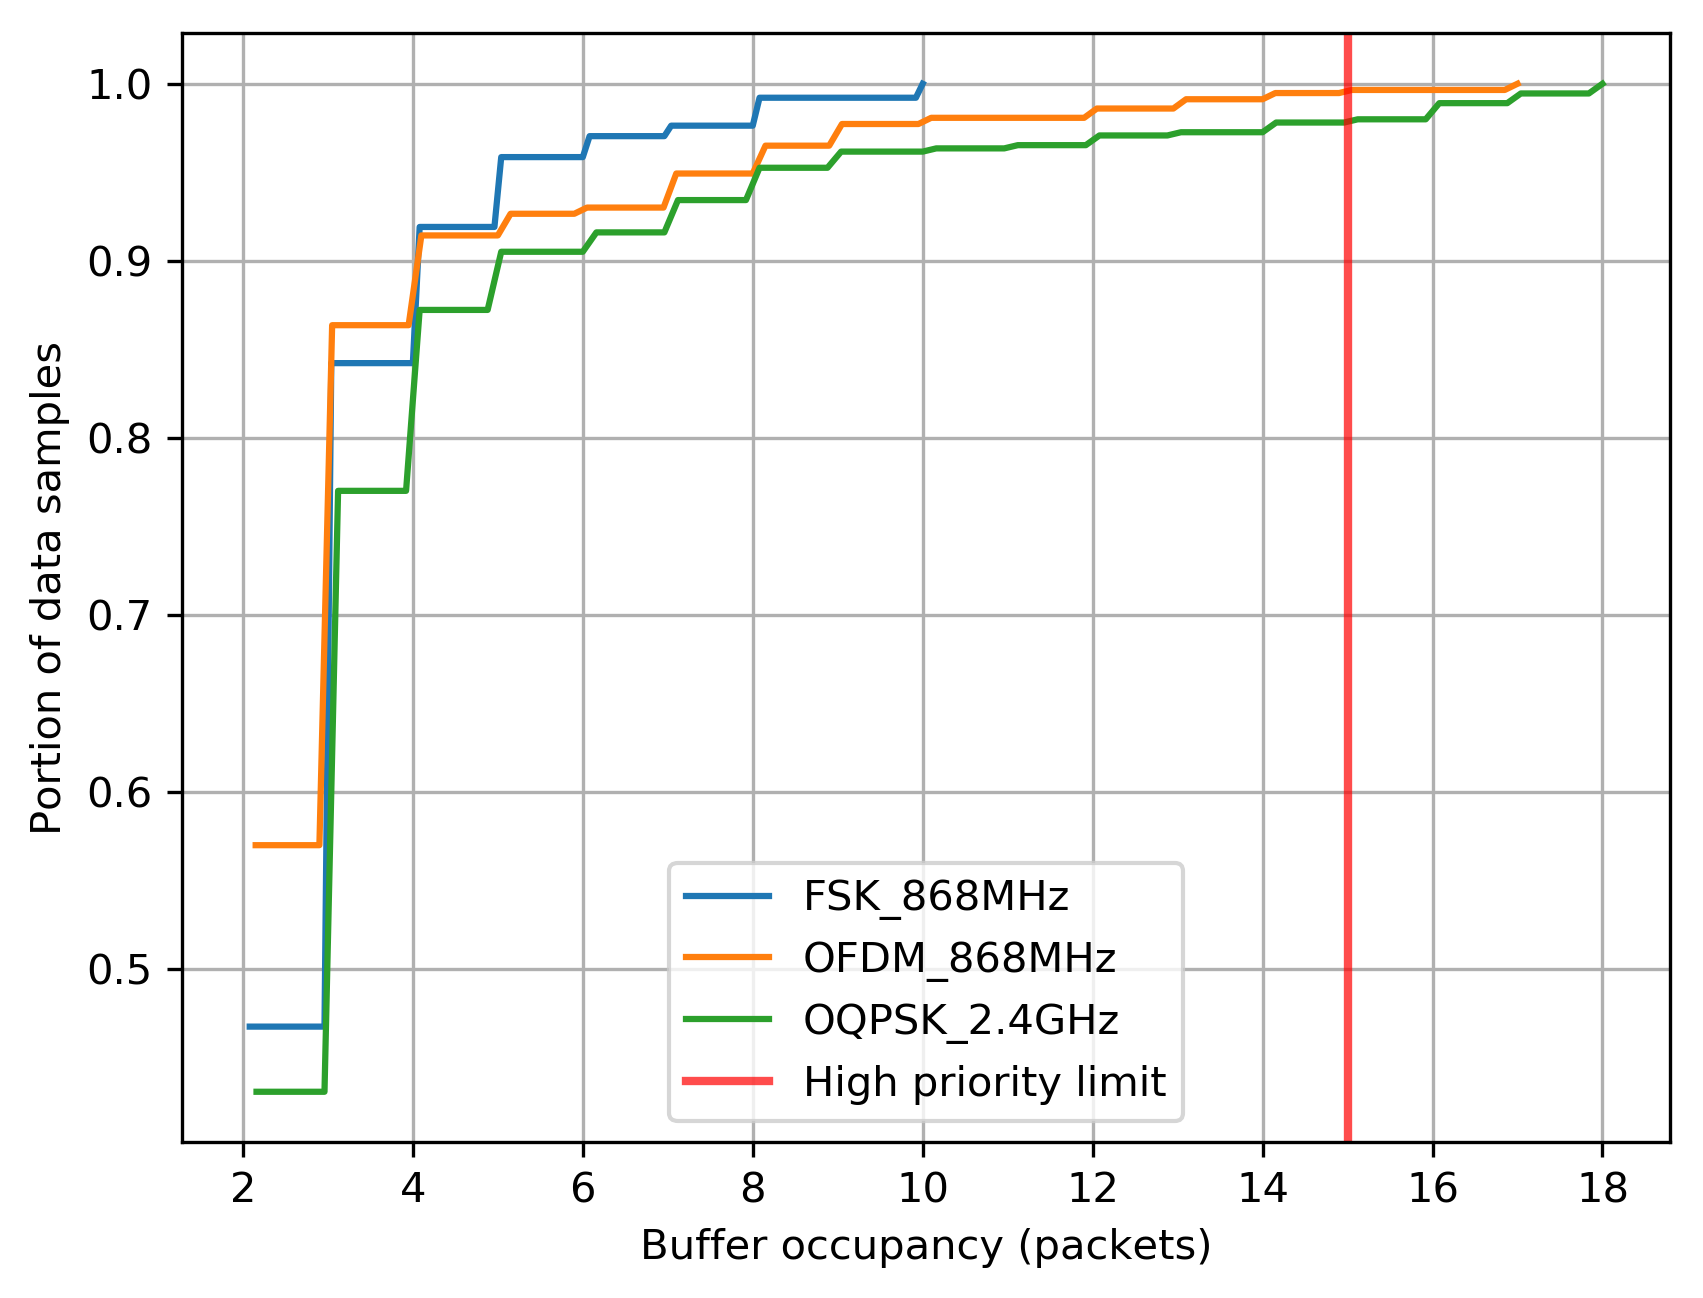
\includegraphics[width=0.49\columnwidth]{maxBufferSize_cdf_plot_full_steady_15}
	\caption{CDF of packet queue occupancy at 15~mins of steady state}
    \label{fig:maxBufferSize_cdf_plot_full_steady_15}
\end{figure}

% pdr because of queue occupancy

One reason behind this PDR is that limitations of the packet queue buffer may impose dropping of newly-arriving packets.
As demonstrated in sub-section \ref{sec:dagroot} a lower link budget PHY layer leads to higher the DAG rank in the network, which translates to more re-transmissions for poor-links or more forwarding at relay nodes. 
Both aspects lead to more packets, on average, remaining in the buffer, either for re-transmission or forwarding.
Therefore, more motes can reach their buffer limitations and consequently drop packets.

% show queue plots. 

For verification, a CDF of maximum packet buffer occupancy is plotted in Fig.~\ref{fig:maxBufferSize_cdf_plot_full_steady_15} for the steady state of the last 15~minutes. 
The queue size for the stack is set to 20 packet entries; however, 5 entries are reserved for high priority packets (IEEE802.15.4e MAC packets).
It can be observed, on one hand, that in nearly 3\% and 1\% of the reports, motes exceed the 15-packet occupancy with \oqpsk\ and \ofdm\ respectively.
On the other hand, \fsk\ maintains a light memory footprint below 10-packets for all the data samples. 
Those values conform to the discrepancies in PDR expressed in table~\ref{tab:pdr_table}. 
Therefore, the higher the link-budget, the lower the chance of packet loss based on packet buffer overflow. 

%------------------------------------------------------------------------------
\subsection{End-to-End Latency}
\label{sec:latency}

% why, how is it measured

This is a significant KPI for IIoT since some traffic can generated by alarm events.
In this case, they need to be detected at the root as soon as possible to minimize safety-risks or equipment damage.
It is measured as difference between ASN in the UDP packet and the ASN of the root at packet reception multiplied by the slot-duration of 40ms.

% impact of phy layer. 

The link-budget of PHY layer is in inverse correlation with the end-to-end latency as observed in Fig.~\ref{fig:latency_time}.
Furthermore, 90\% of the reports are late by nearly 10, 25, and 35~seconds for \fsk\ , \ofdm\ , and \oqpsk\ respectively, as observed in Fig.~\ref{fig:latency_cdf}.
Fig.~\ref{fig:latency_pdf} shows that the latency distribution is ``wider'' at lower link budget.
On one hand, the tail of the distribution with \oqpsk\  reaches more than 50~seconds whereas the center of the distribution is around 25~seconds.
On the other hand, the overwhelming majority of latency reports with \fsk\ is centered around 5~seconds.

% explanation

This phenomena is related to the increase in path-costs in the network (expressed by the DAG rank).
As previously demonstrated in subsection \ref{sec:dagroot}, lower link-budget leads to higher DAG rank which translates to a combination of larger-number of hops and/or re-transmission count.
This leads to an increase in end-to-end latency distribution, especially for the nodes at the absolute bottom of the routing tree. 
Therefore, at higher link budget at the PHY-layer, the distribution of the end-to-end latency is improved for the network.

\begin{figure}
	\centering
	\begin{subfigure}{0.49\columnwidth}
    	\centering
    	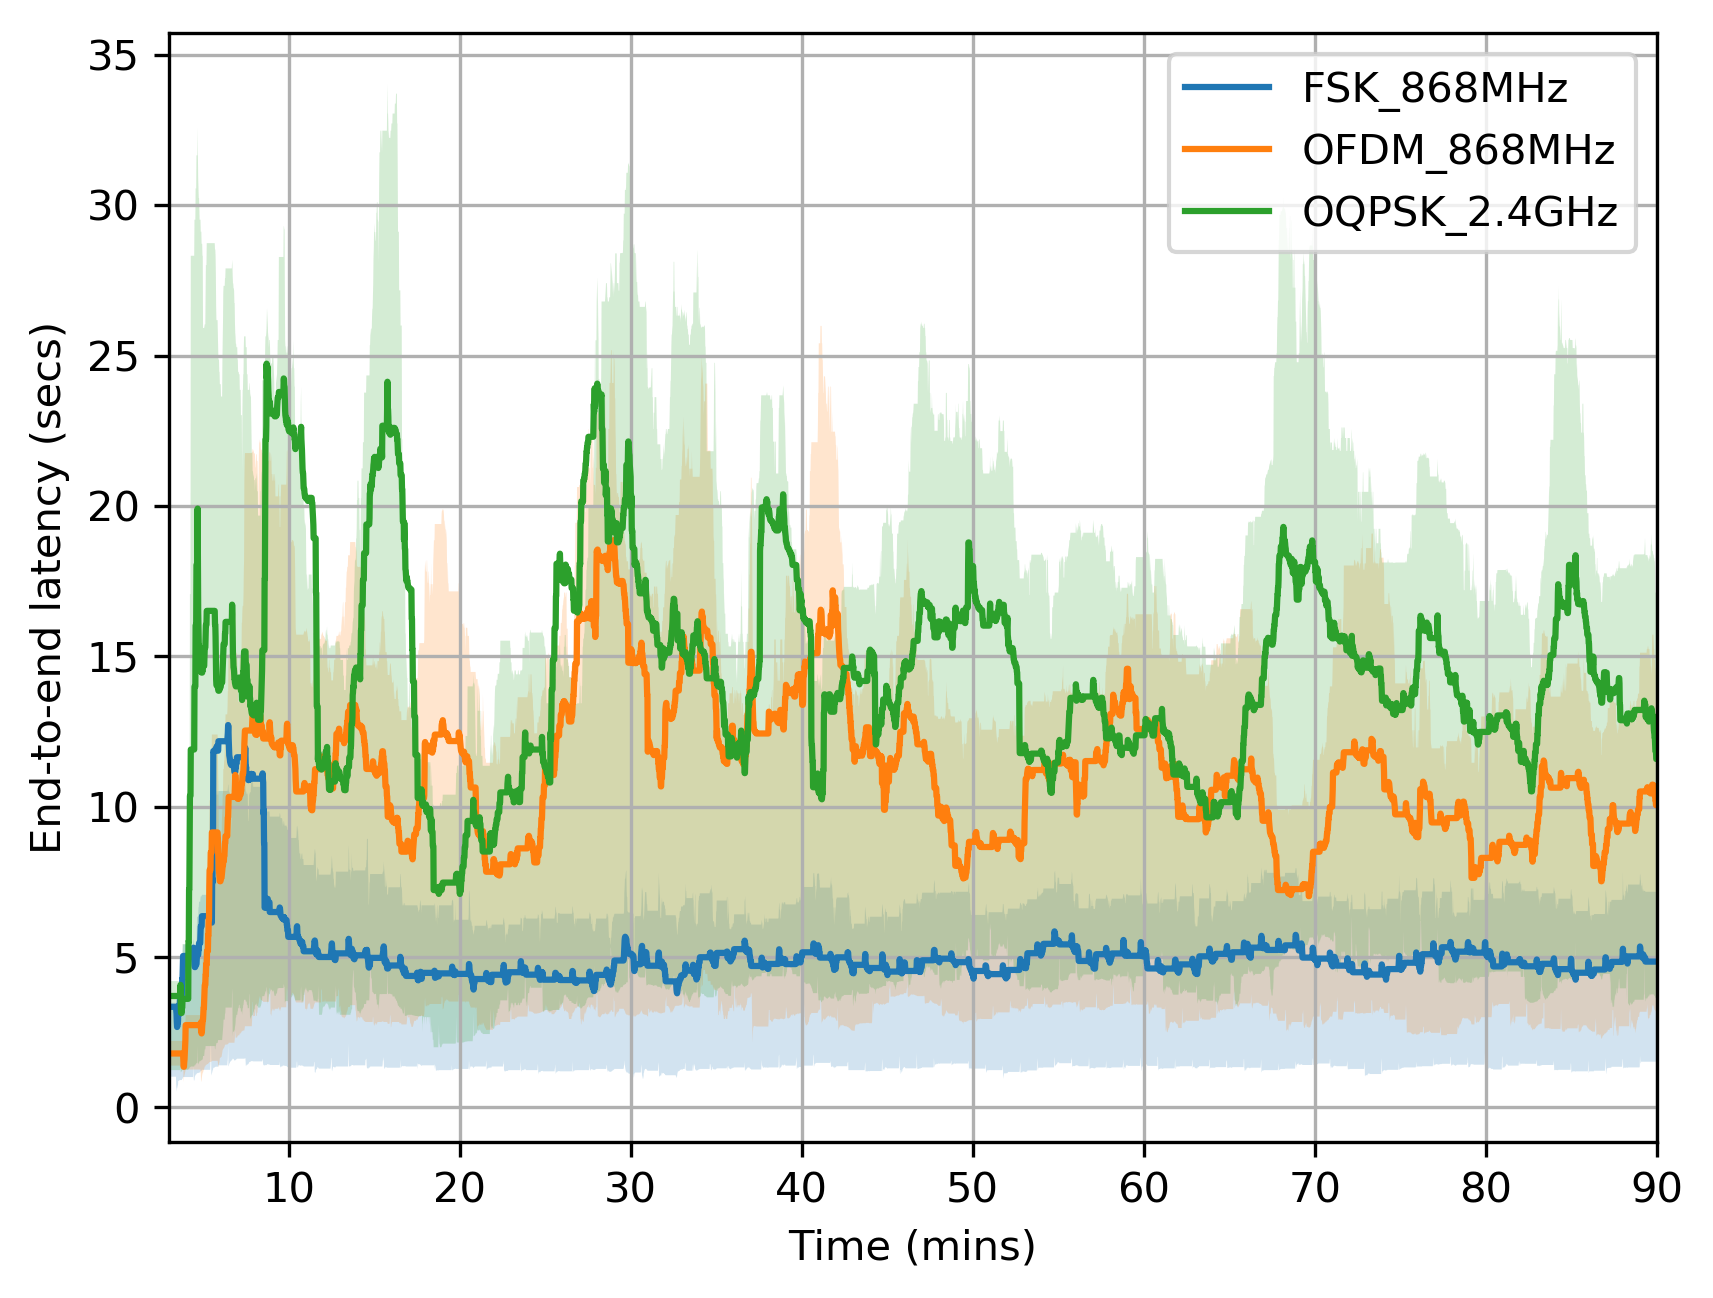
\includegraphics[width=1.00\columnwidth]{latency_time}
        \subcaption{Mean and inter-quartile range of measurements in the time domain }
        \label{fig:latency_time}
	\end{subfigure}
	\begin{subfigure}{0.49\columnwidth}
		\centering
    	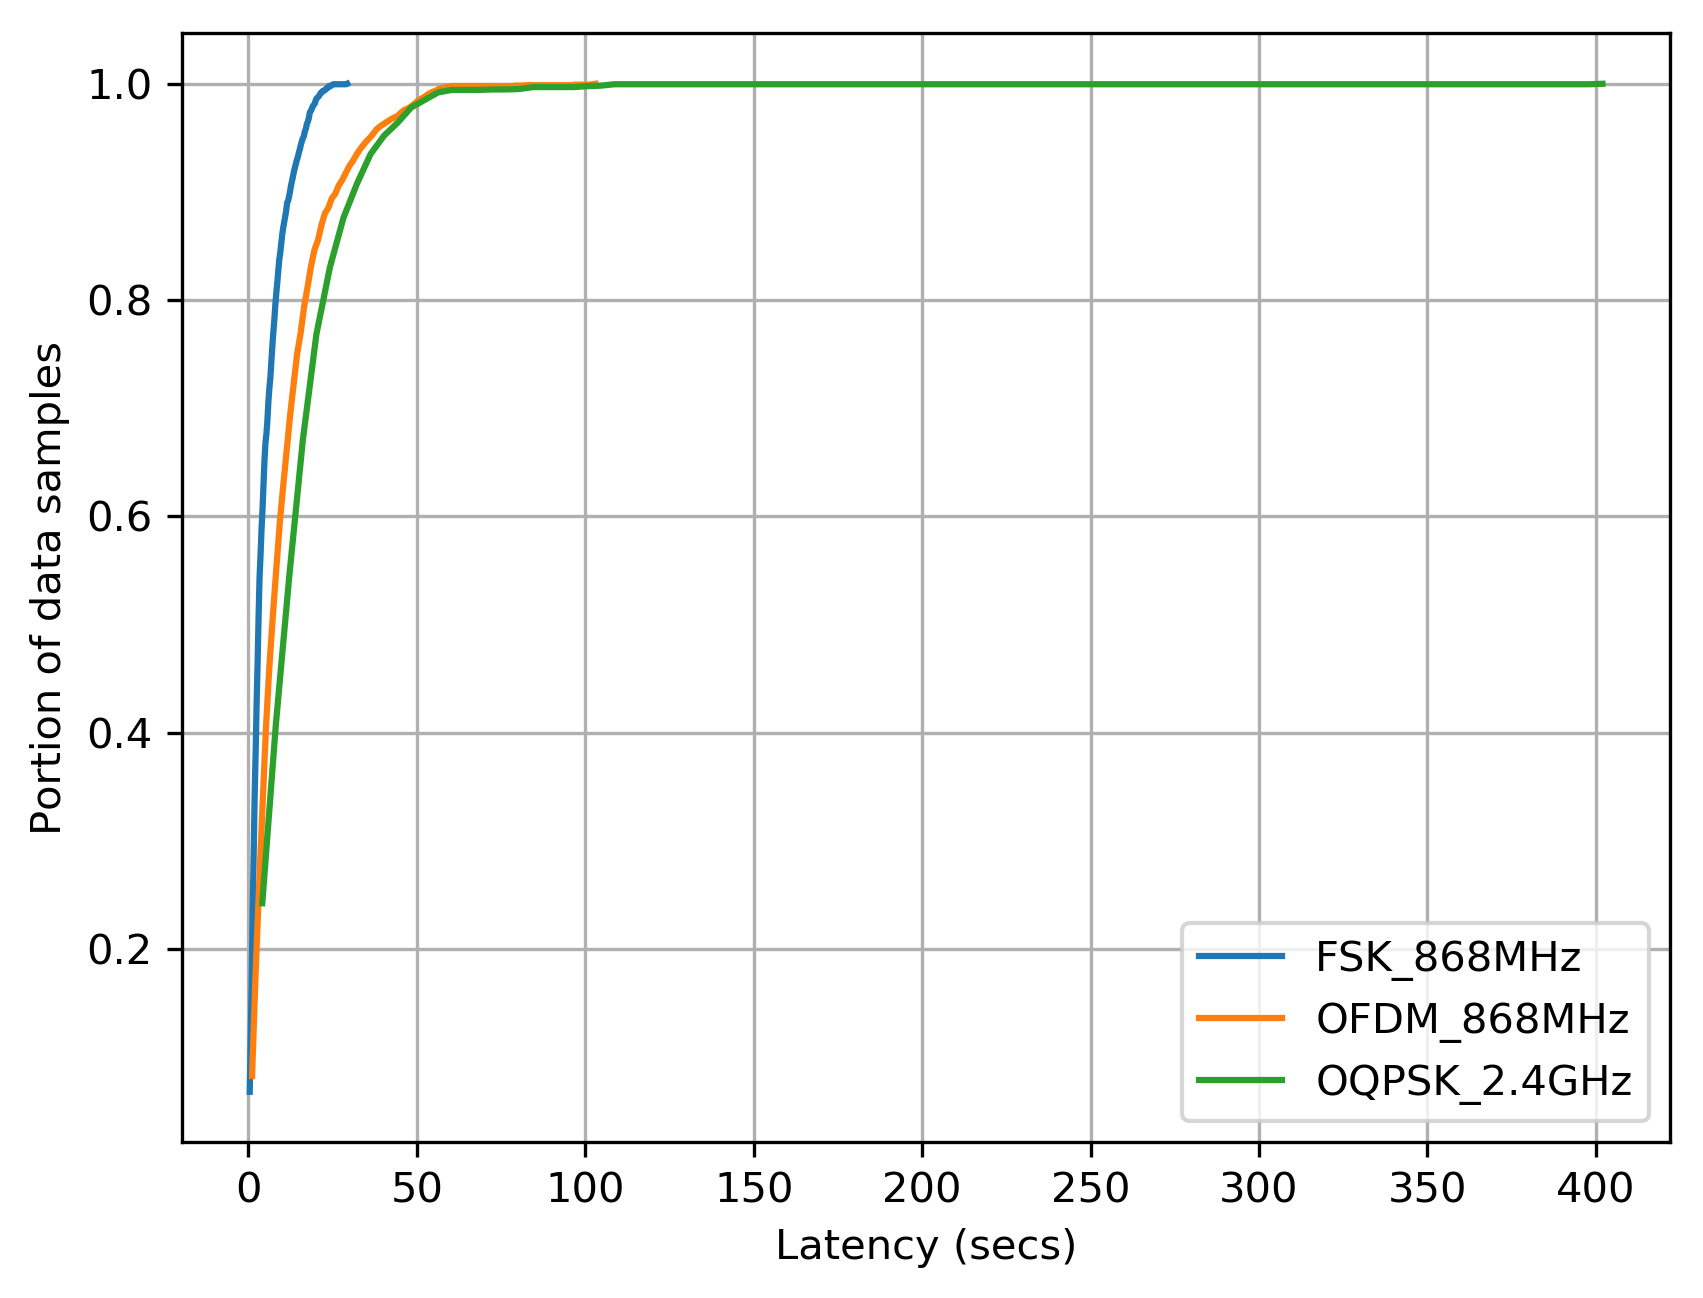
\includegraphics[width=1.00\columnwidth]{latency_cdf}
    	\subcaption{CDF of  the measurements for the network at steady state }
        \label{fig:latency_cdf}
	\end{subfigure}
	\begin{subfigure}{0.49\columnwidth}
		\centering
    	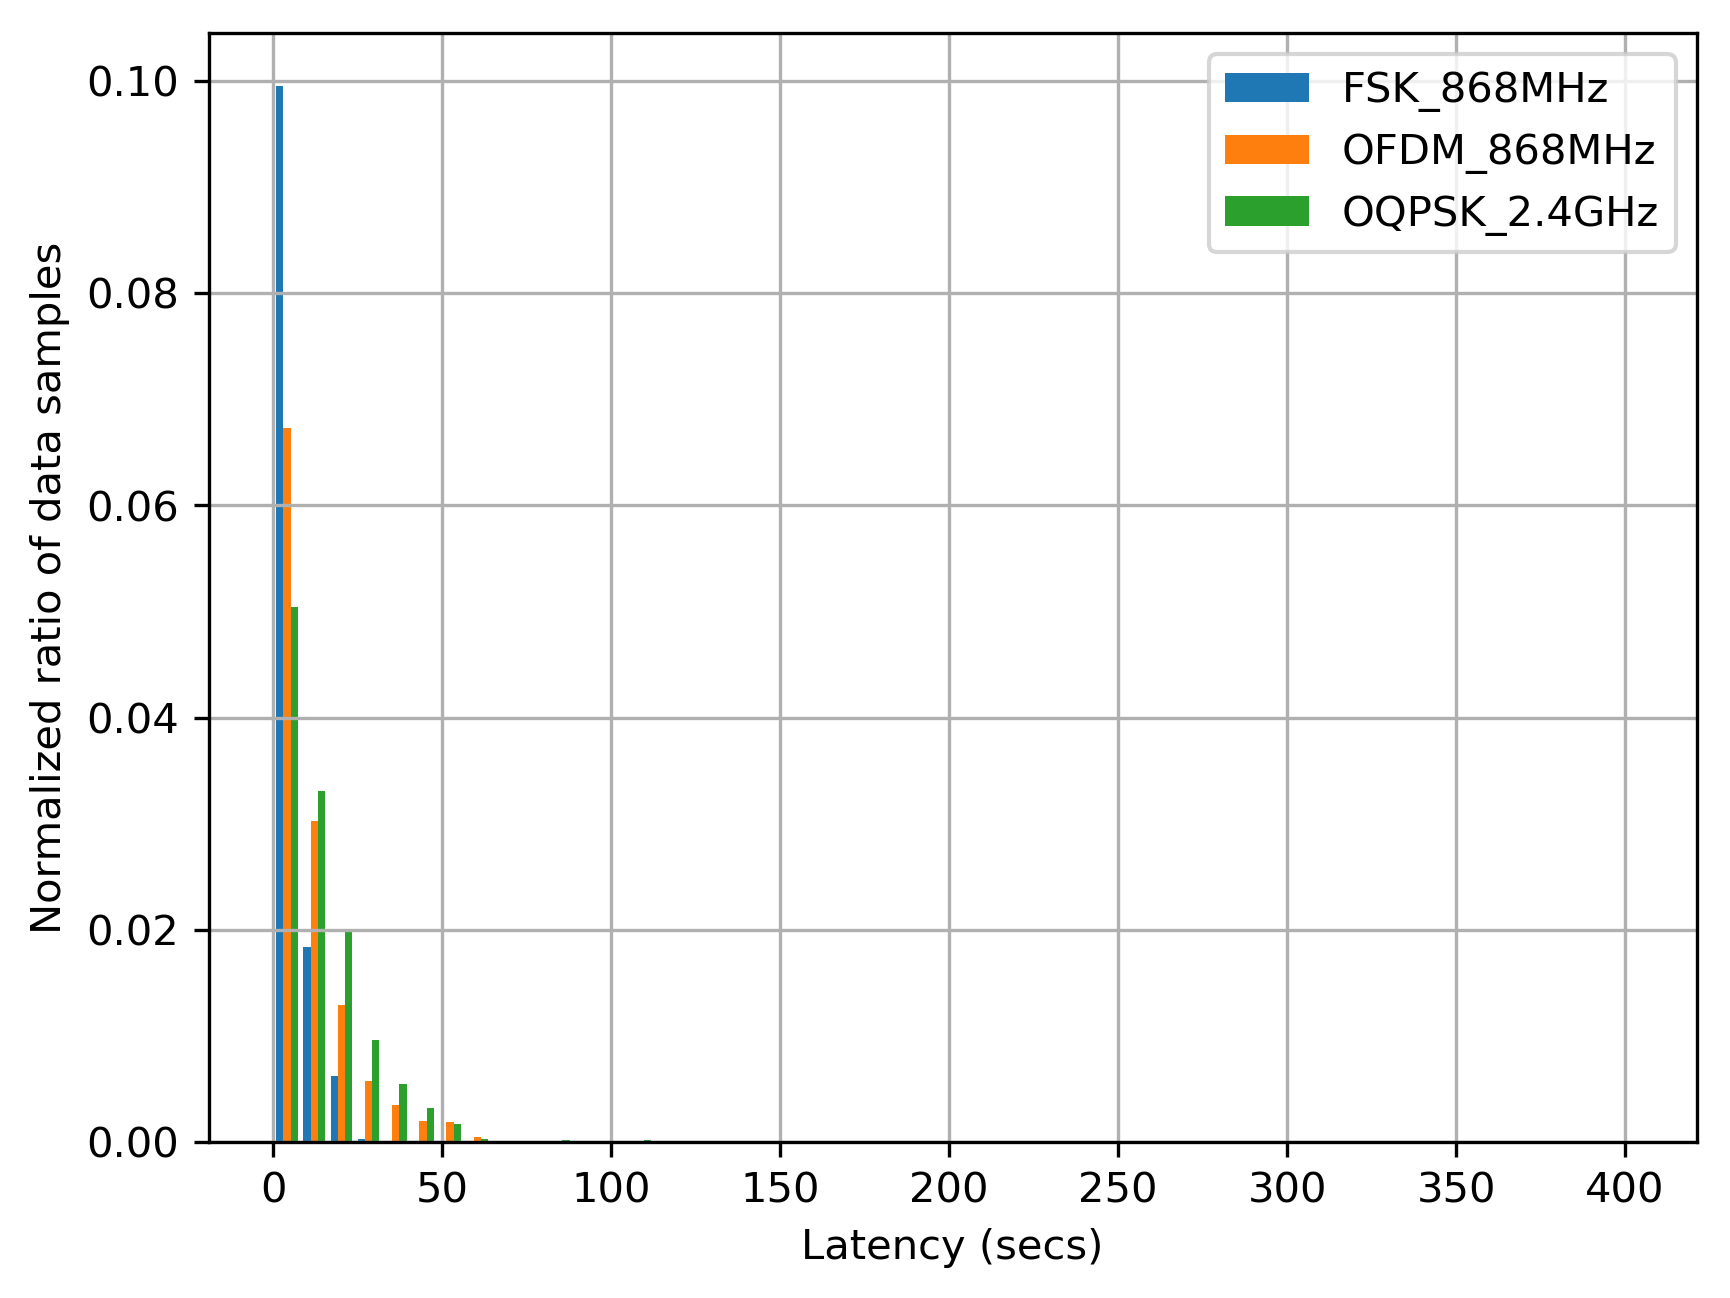
\includegraphics[width=1.00\columnwidth]{latency_pdf}
    	\subcaption{PDF of  the measurements for the network at steady state}
    	\label{fig:latency_pdf}
	\end{subfigure}
	\caption{
	    Reported end-to-end latency in the network.
	    The higher the link budget, the lower the latency in the network.
	}
	\label{fig:latency_all}
\end{figure}

%------------------------------------------------------------------------------
\subsection{Battery Lifetime}
\label{sec:battery_lifetime}

% why important? measured how?

This KPI is essential to determine the real cost of running the network because operational expenditure (OpEx) is needed for battery replacement during network operation. 
The OpEx includes battery costs as well as the labor cost, which could be significant for equipment located in hard-to-reach or remote areas. 
It is calculated based on the radio DC and the radio power consumption in transmit and receive states. 
Three measurements are captured in the firmware: 1) total time the radio is on $T_{on}$, 2) and total time the radio is in transmit state $T_{tx}$ , and 3) the total time the network is running $T_{total}$. 

\begin{figure}
	\centering
	\begin{subfigure}{0.49\columnwidth}
    	\centering
    	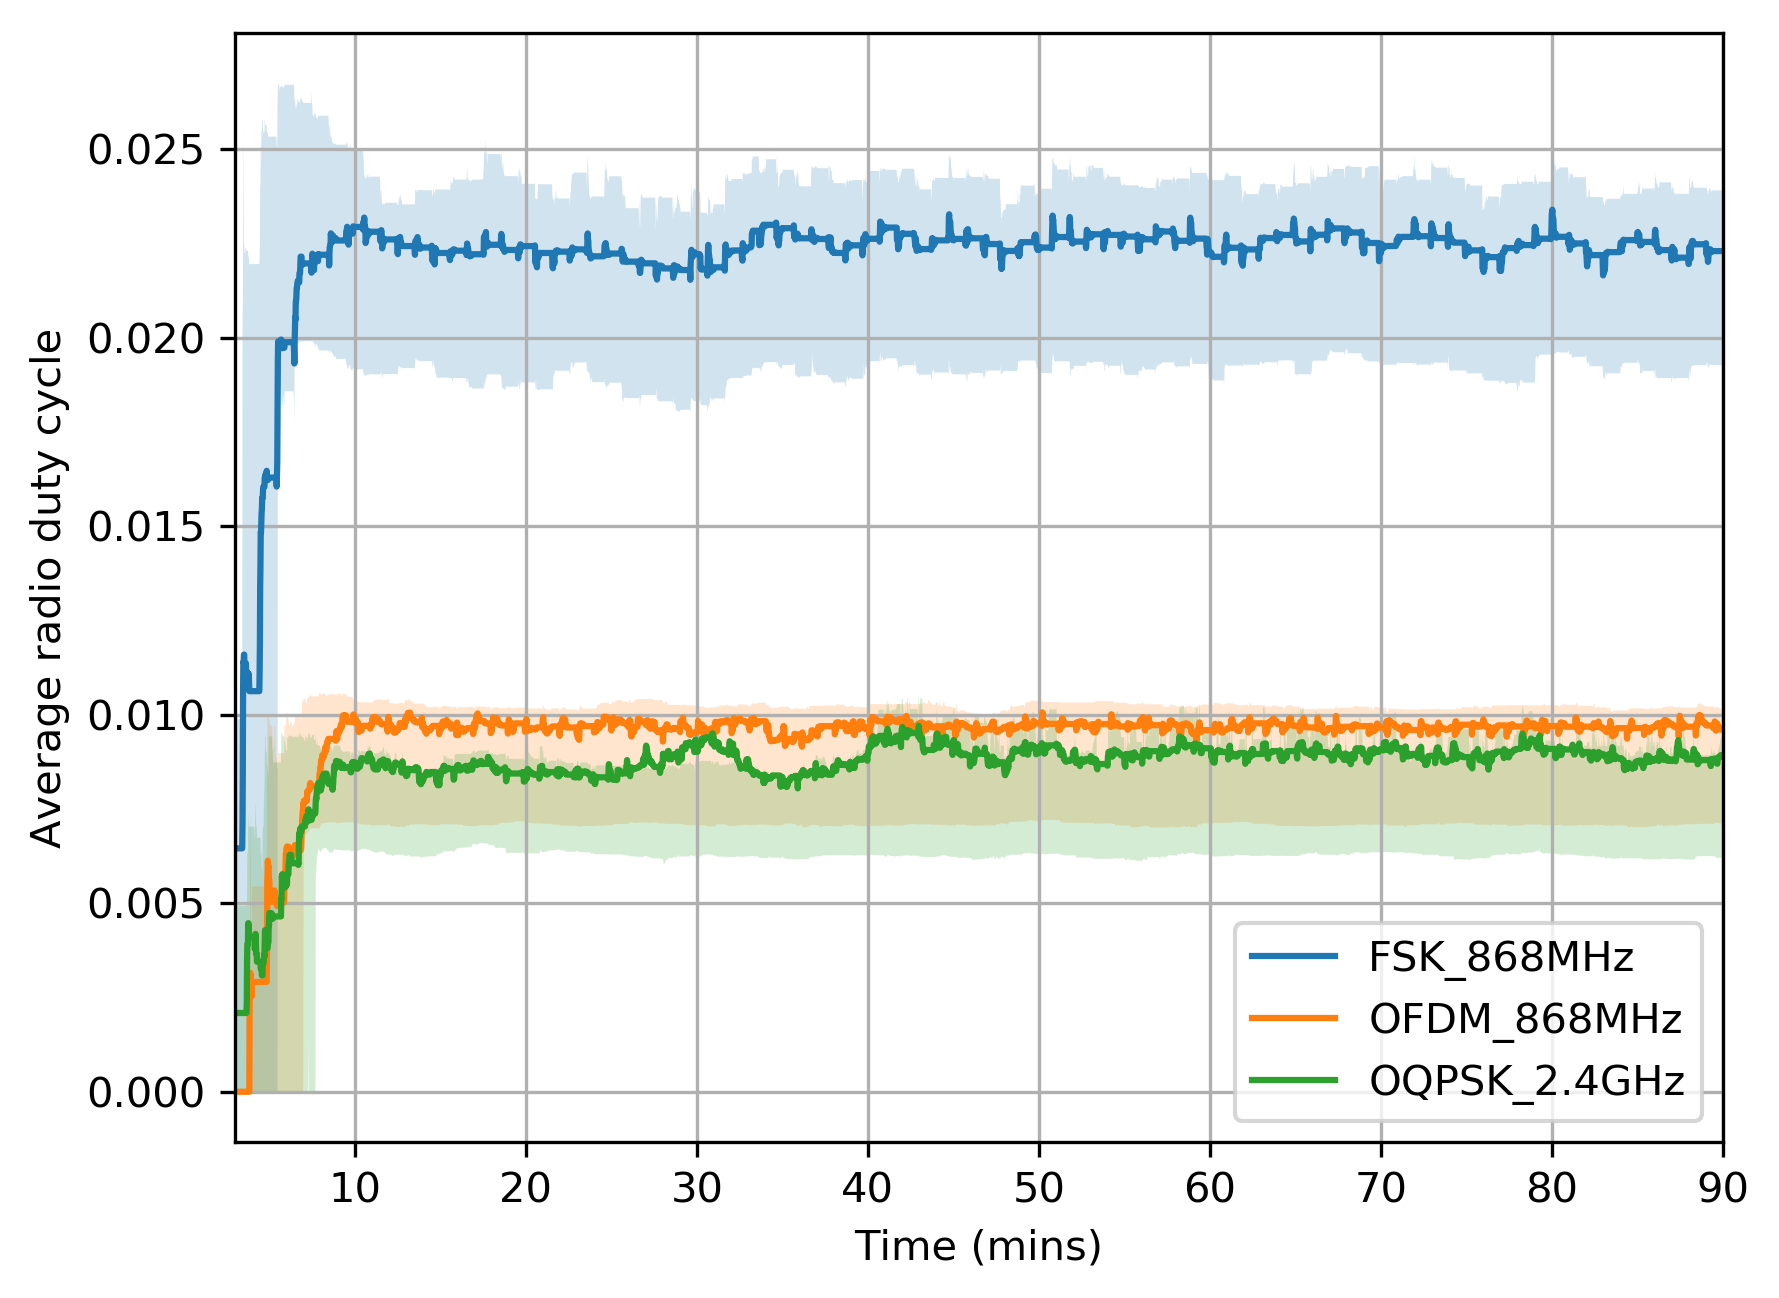
\includegraphics[width=1.00\columnwidth]{dutyCycle_time}
        \subcaption{Mean and inter-quartile range of measurements in the time domain }
        \label{fig:dutyCycle_time}
	\end{subfigure}
	\begin{subfigure}{0.49\columnwidth}
		\centering
    	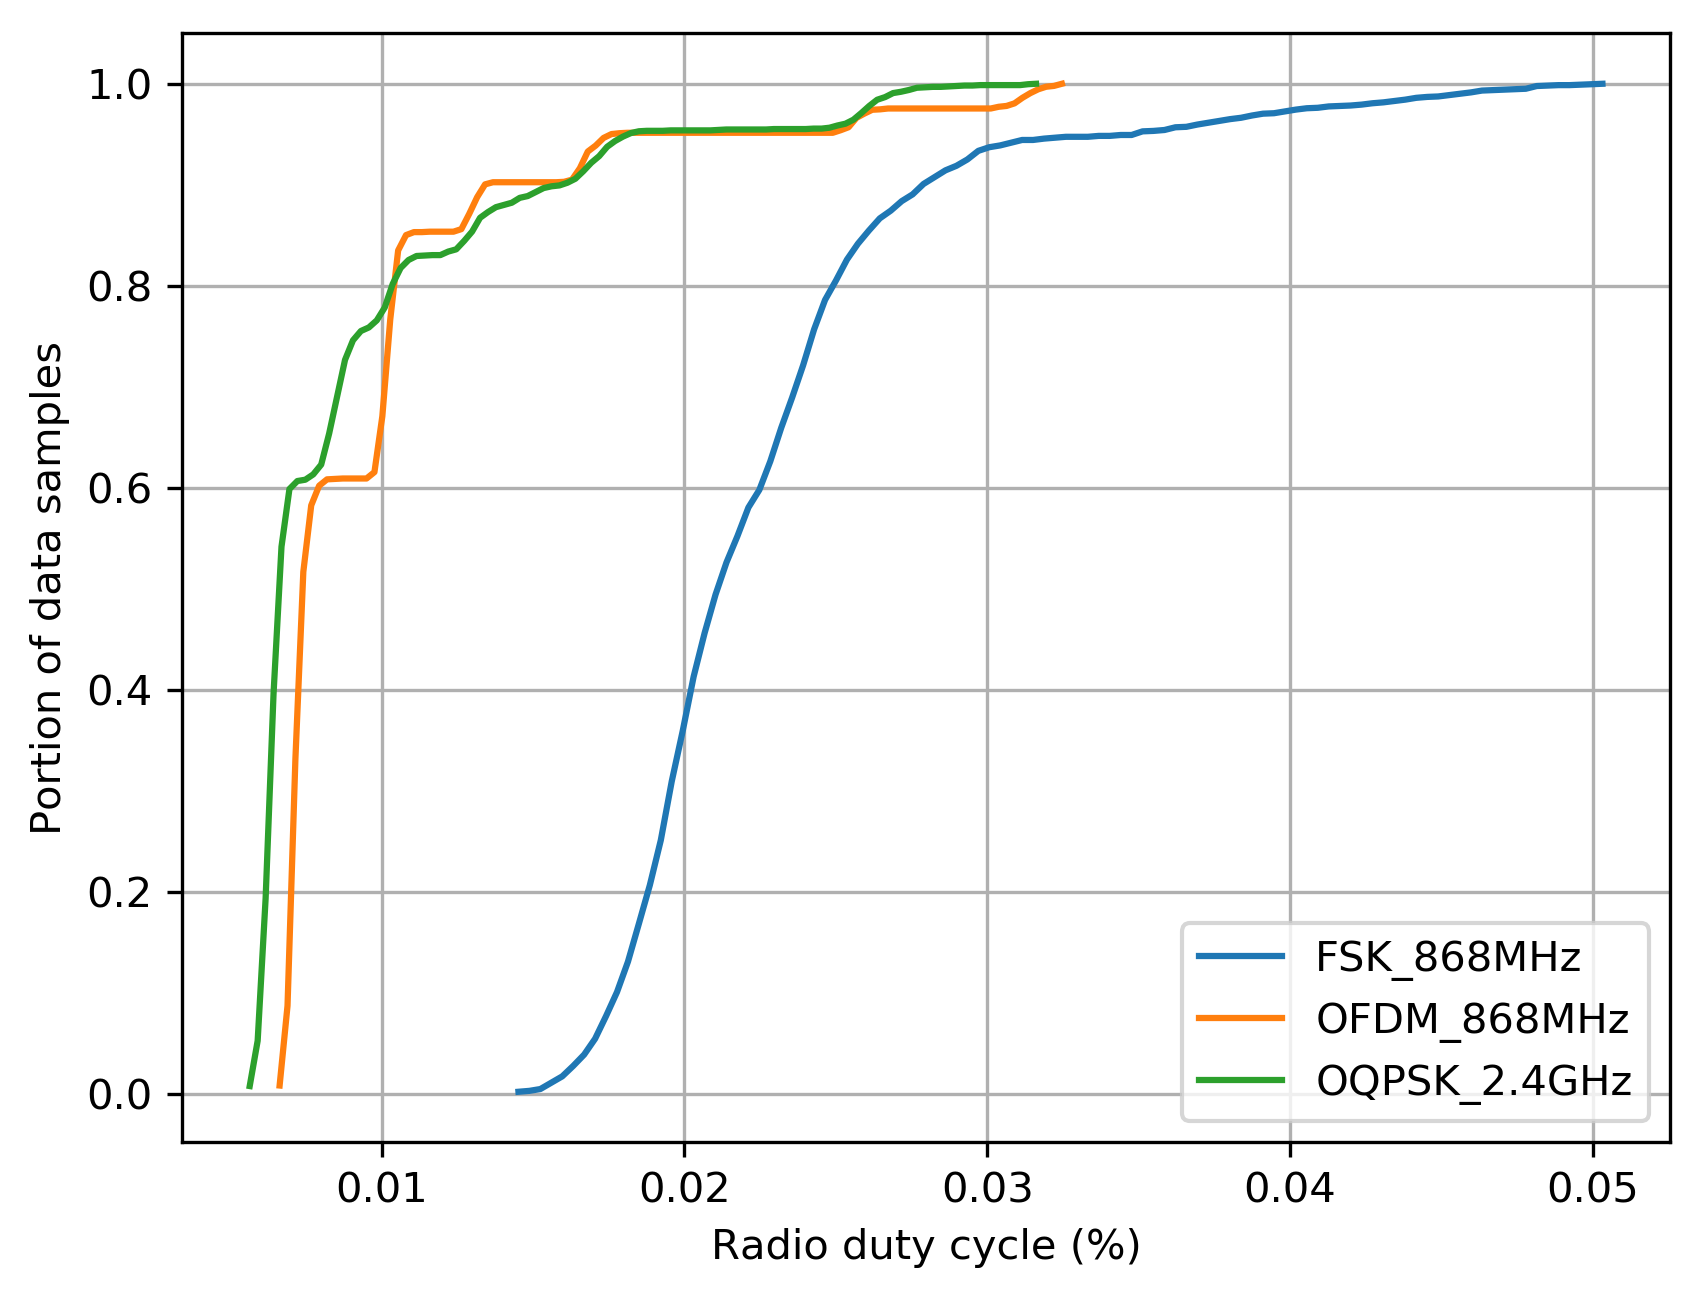
\includegraphics[width=1.00\columnwidth]{dutyCycle_cdf}
    	\subcaption{CDF of  the measurements for the network at steady state }
        \label{fig:dutyCycle_cdf}
	\end{subfigure}
	\begin{subfigure}{0.49\columnwidth}
		\centering
    	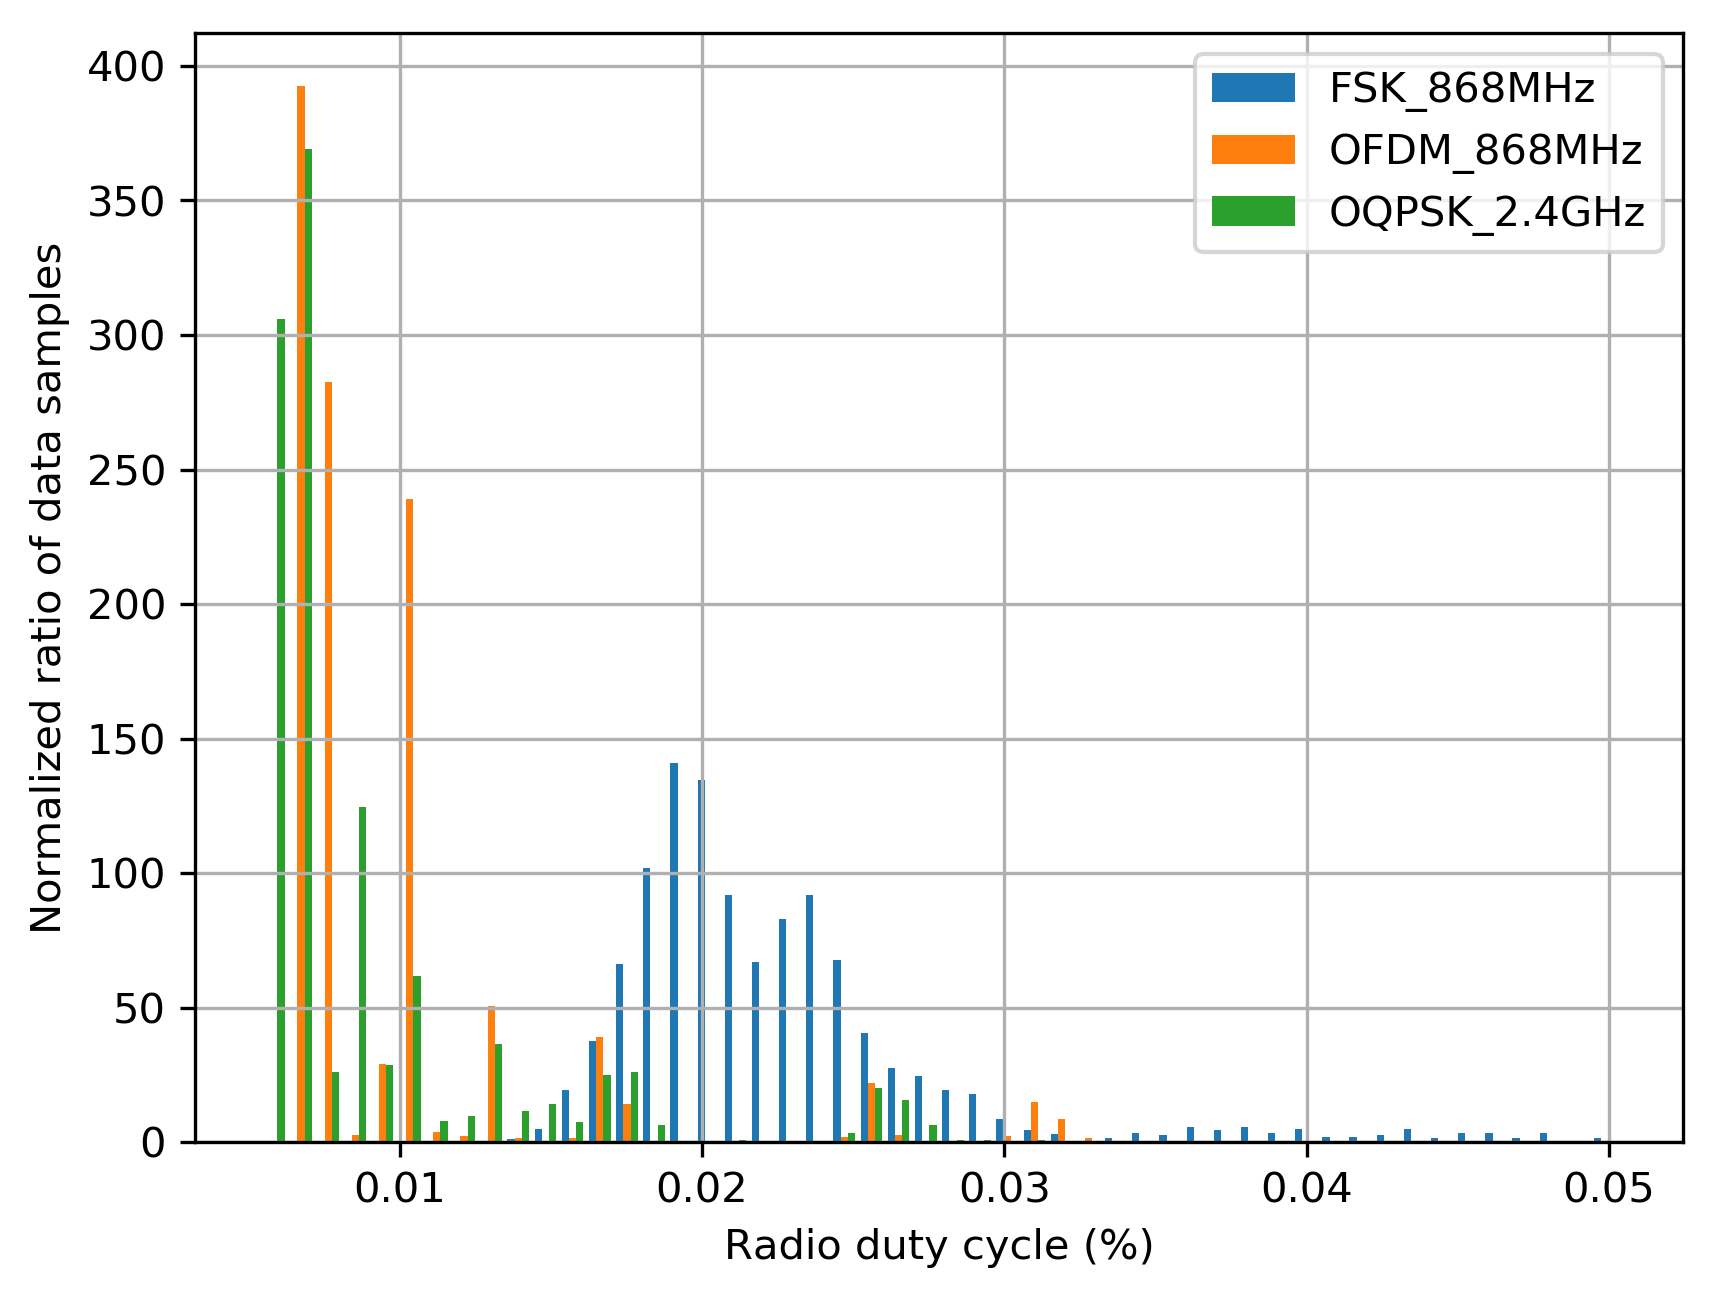
\includegraphics[width=1.00\columnwidth]{dutyCycle_pdf}
    	\subcaption{PDF of  the measurements for the network at steady state  }
    	\label{fig:dutyCycle_pdf}
	\end{subfigure}
	\caption{
	    Reported radio duty cycle in the network.
	    Lower bit-rate and SPI communications overhead leads to higher duty cycle and power consumption.
	}
	\label{fig:dutyCycle_all}
\end{figure}

Radio DC is calculated as: $DC=T_{on}/T_{total}$ and is shown in Fig.~\ref{fig:dutyCycle_all}.
As expected, bit-rate is inversely correlated with DC. 
However, the DC of \fsk\ is larger than the other two options by more than a factor of 2, even though it is slower than \oqpsk\ and \ofdm\ by factors of 5 and 8 respectively. 
Similarly, \ofdm\ is nearly 3 times as high as  \oqpsk\ in bit-rate, yet it is sightly higher in DC.
This observation is verified in CDF in Fig.~\ref{fig:dutyCycle_cdf} and Fig.~\ref{fig:dutyCycle_pdf} where 90\% of the motes are at nearly 0.015\% for \oqpsk\ and \ofdm\ and at 2 orders of magnitude for \fsk\. 
This is attributed to two reasons.
First, the higher DAG-rank distribution of \oqpsk\ and \ofdm\ -- as observed in Fig.~\ref{fig:dagrank_all}-- translates to more time on air due to either re-transmissions or forwarding over longer hops or both.
Second, execution of driver commands for \texttt{AT86rf215} requires an additional time for SPI communications overhead which reaches up to 1~ms, as demonstrated in Fig.~\ref{fig:openradio}.

\begin{table}
    \centering
    \begin{tabular}{|l|l|l|l|l|l|l|l|l|}
        \hline
                & DC     & $DC_{tx}$ & $DC_{rx}$ & $P_{tx}^{max}$ (w) & $P_{rx}^{max}$(w) & Supply voltage (v) & Energy per day (wh) & \textbf{Estimated days} \\ \hline
        \fsk\   & 0.021  & 0.0025    & 0.0185    & 62             & 28             & 2.5            & 0.0141174           & 580.8435       \\ \hline
        \ofdm\  & 0.0075 & 0.000375  & 0.007125  & 62             & 28             & 2.5            & 0.00325035          & 2522.805       \\ \hline
        \oqpsk\ & 0.0065 & 0.0005    & 0.006     & 24             & 20             & 3              & 0.00148608          & 5517.873       \\ \hline
    \end{tabular}
    \caption{Battery lifetime for each configuration}
    \label{tab:energy_table}
\end{table}

% OpEx reasons. 

Radio power consumption in both Tx and Rx states is noted in table \ref{tab:energy_table}.
Since $T_{tx}$ and $T_{on}$ are known, $T_{rx}$ is estimated as $T_{on}-T_{rx}$.
Then $DC_{tx}=T_{tx}/T_{total}$ and $DC_{rx}=T_{rx}/T_{total}$.
Assuming two AA batteries with total 8.2 wh capacity, the battery lifetime of each configuration is estimated in table \ref{tab:energy_table}.
It is observed that \oqpsk\ extends the battery life by nearly a factor of 5 more than \ofdm\ and by nearly a factor of 10  more than \fsk\ .
Therefore, despite the demonstrated range, reliability, and latency advantages of \fsk\ and \ofdm\ respectively, their utilization leads to incurred significant network OpEx (as well as environmental bulk battery waste).
This practical aspect of performance may deem a network unfit for deployment simply for budget reasons, even though it is highly reliable. 

%==============================================================================
\section{Discussion}
\label{sec:discussion}

\begin{table}
    \centering
    \begin{tabular}{|l|l|l|l|l|}
        \hline
                & 90\% Network formation & Battery lifetime & 90\% Latency  &  Reliability   \\ \hline
        \fsk\   & 7~mins                 & 580~days      & 10~secs       & 100\%             \\ \hline
        \ofdm\  & 9~mins                 & 2522~days     & 25~secs       & 99.84\%           \\ \hline
        \oqpsk\ & 11~mins                 & 5517~days     & 35~secs       & 98.08\%           \\ \hline
    \end{tabular}
    \caption{6TiSCH performance ranking for each setting}
    \label{tab:summary}
\end{table}

% summary of the performance for each KPI

Results demonstrate that there is ``no free lunch'' for the choice of PHY layer since no single option is best according to all KPIs.
Table~\ref{tab:summary} provides a summary of the rankings of the three options according to each KPI.
First, \fsk\ leads to discovery of most neighbors and lowest DAG rank distribution.
In turn, it leads to the fastest network formation, highest end-to-end reliability, and the lowest end-to-end latency; yet it shortens network battery lifetime by nearly a factor of 10 compared to \oqpsk\. 
It also risks neighbor table overflow in high density deployments.
Second, \oqpsk\ leads to discovery of the least neighbors and highest DAG rank distribution in the network.
It also risks packet-buffer overflow potentially due to storage needed for re-transmissions and forwarding.
In turn, this leads to the slowest network formation, the lowest end-to-end reliability, and the highest end-to-end latency.
However, it provides the best battery lifetime of the network. 
Finally, \ofdm\ demonstrates an intermediate network formation time, end-to-end reliability, and end-to-end latency; yet  it decreases the battery lifetime by a factor of 5 compared to \oqpsk.

% future work

These findings motivate future work to integrate multiple PHY-layers in the 6TiSCH protocol stack.
This allows an agile performance of the protocol stack as it adapts the PHY layer at link-level depending on link quality.
Therefore, this has a potential as a reasonable compromise among the advantages and disadvantages of each option and an overall improved KPI evaluations. 

% \bibliographystyle{IEEEtran}
\bibliography{rady20free}

\end{document}